\pdfoutput=1

\documentclass[runningheads]{llncs}

% ---------------------------------------------------------------
% Include basic ECCV package
 
% TODO REVIEW: Insert your submission number below by replacing '*****'
% TODO FINAL: Comment out the following line for the camera-ready version
% \usepackage[review,year=2024,ID=8270]{eccv}
% TODO FINAL: Un-comment the following line for the camera-ready version
% \usepackage{eccv}

% OPTIONAL: Un-comment the following line for a version which is easier to read
% on small portrait-orientation screens (e.g., mobile phones, or beside other windows)
\usepackage[mobile]{eccv}


% ---------------------------------------------------------------
% Other packages

% Commonly used abbreviations (\eg, \ie, \etc, \cf, \etal, etc.)
\usepackage{eccvabbrv}

% Include other packages here, before hyperref.
\usepackage{graphicx}
\usepackage{booktabs}

% The "axessiblity" package can be found at: https://ctan.org/pkg/axessibility?lang=en
\usepackage[accsupp]{axessibility}  % Improves PDF readability for those with disabilities.

% CUSTOM PACKAGES
\usepackage[table]{colortbl}
\usepackage{verbatim}
\usepackage{setspace}


% ---------------------------------------------------------------
% Hyperref package

% It is strongly recommended to use hyperref, especially for the review version.
% Please disable hyperref *only* if you encounter grave issues.
% hyperref with option pagebackref eases the reviewers' job, but should be disabled for the final version.
%
% If you comment hyperref and then uncomment it, you should delete
% main.aux before re-running LaTeX.
% (Or just hit 'q' on the first LaTeX run, let it finish, and you
%  should be clear).

% TODO FINAL: Comment out the following line for the camera-ready version
% \usepackage[pagebackref,breaklinks,colorlinks,citecolor=eccvblue]{hyperref}
% TODO FINAL: Un-comment the following line for the camera-ready version
\usepackage{hyperref}

% Support for ORCID icon
\usepackage{orcidlink}


%
% Examples:
%
% \addeditor{vincent}{VL}{0.0, 0.5, 0.0}
% adds the following commands:
% \vincent{text}, \vincentrmk{remark}, and \vincentrpl{newtext}{oldtext}
% 
% You can also use \todo{add this}
%
% Use:
% \showeditstrue
% and:
% \showeditsfalse
% to show or hide the edits

% \textvars{pose,rot}
% adds the following commands:
% \pose, which is replaced by \text{pose} and
% \rot, which is replaced by \text{rot}


% \moretextwithfigures
% forces LaTeX to put text to pages that would normally contain only
% figures

% Use
% \calA for \mathcal{A}, etc.
% \bA for \textbf{A}, etc.
% \ba for \textbf{a}, etc.
% \IR for \mathds{R}, etc.

\usepackage{dsfont}
\usepackage{etoolbox}
\usepackage{color}


\newif\ifshowedits

\newcommand{\addeditor}[3]{%
  \definecolor{#1color}{rgb}{#3}
  \expandafter\newcommand\csname #1\endcsname[1]{%
  \ifshowedits
    {\color{#1color} ##1}%
  \else
    {##1}%
  \fi
  }%
  \expandafter\newcommand\csname #1rmk\endcsname[1]{%
  \ifshowedits
    {\color{#1color} {\bf [#2: ##1]}}
  \fi
  }%
  \expandafter\newcommand\csname #1rpl\endcsname[2]{%
  \ifshowedits
    {\color{#1color} ##1 \sout{##2}}
  \else
    {##1}
  \fi
  }%
}

\newcommand\todo[1]{%
  \ifshowedits
    {\color{red} {\bf #1}}
  \fi
}

%%%%%%%%%%%%%%%%%%%%%%%%%%%%%%%%%%%%%%%%%%%%%%%%%%%%%%%%%%%%%%%%%%%%%%%%%%%%%%%%

\newcommand{\createtextvar}[1]{
  \expandafter\newcommand\csname #1\endcsname{%
  {\text{#1}}
}%
}
%
\newcommand{\textvars}[1]{\forcsvlist{\createtextvar}{#1}}


%%%%%%%%%%%%%%%%%%%%%%%%%%%%%%%%%%%%%%%%%%%%%%%%%%%%%%%%%%%%%%%%%%%%%%%%%%%%%%%%

\newcommand{\moretextwithfigures}{
\renewcommand{\topfraction}{1}
\renewcommand{\dbltopfraction}{1}
\renewcommand{\bottomfraction}{1}
\renewcommand{\textfraction}{.0}
\renewcommand{\floatpagefraction}{1}
\renewcommand{\dblfloatpagefraction}{1}
}

%%%%%%%%%%%%%%%%%%%%%%%%%%%%%%%%%%%%%%%%%%%%%%%%%%%%%%%%%%%%%%%%%%%%%%%%%%%%%%%%

\newcommand{\mycomment}[1]{}

%%%%%%%%%%%%%%%%%%%%%%%%%%%%%%%%%%%%%%%%%%%%%%%%%%%%%%%%%%%%%%%%%%%%%%%%%%%%%%%%

\newcommand{\calA}{{\cal A}}
\newcommand{\calB}{{\cal B}}
\newcommand{\calC}{{\cal C}}
\newcommand{\calD}{{\cal D}}
\newcommand{\calE}{{\cal E}}
\newcommand{\calF}{{\cal F}}
\newcommand{\calG}{{\cal G}}
\newcommand{\calH}{{\cal H}}
\newcommand{\calI}{{\cal I}}
\newcommand{\calJ}{{\cal J}}
\newcommand{\calK}{{\cal K}}
\newcommand{\calL}{{\cal L}}
\newcommand{\calM}{{\cal M}}
\newcommand{\calN}{{\cal N}}
\newcommand{\calO}{{\cal O}}
\newcommand{\calP}{{\cal P}}
\newcommand{\calQ}{{\cal Q}}
\newcommand{\calR}{{\cal R}}
\newcommand{\calS}{{\cal S}}
\newcommand{\calT}{{\cal T}}
\newcommand{\calU}{{\cal U}}
\newcommand{\calV}{{\cal V}}
\newcommand{\calW}{{\cal W}}
\newcommand{\calX}{{\cal X}}
\newcommand{\calY}{{\cal Y}}
\newcommand{\calZ}{{\cal Z}}

%%%%%%%%%%%%%%%%%%%%%%%%%%%%%%%%%%%%%%%%%%%%%%%%%%%%%%%%%%%%%%%%%%%%%%%%%%%%%%%%

\newcommand{\ba}{{\bf a}}
\newcommand{\bb}{{\bf b}}
\newcommand{\bc}{{\bf c}}
\newcommand{\bd}{{\bf d}}
\newcommand{\be}{{\bf e}}
\newcommand{\bbf}{{\bf f}}  % \bf is a LaTeX command...
\newcommand{\bg}{{\bf g}}
\newcommand{\bh}{{\bf h}}
\newcommand{\bi}{{\bf i}}
\newcommand{\bj}{{\bf j}}
\newcommand{\bk}{{\bf k}}
\newcommand{\bl}{{\bf l}}
\newcommand{\bm}{{\bf m}}
\newcommand{\bn}{{\bf n}}
\newcommand{\bo}{{\bf o}}
\newcommand{\bp}{{\bf p}}
\newcommand{\bq}{{\bf q}}
\newcommand{\br}{{\bf r}}
\newcommand{\bs}{{\bf s}}
\newcommand{\bt}{{\bf t}}
\newcommand{\bu}{{\bf u}}
\newcommand{\bv}{{\bf v}}
\newcommand{\bw}{{\bf w}}
\newcommand{\bx}{{\bf x}}
\newcommand{\by}{{\bf y}}
\newcommand{\bz}{{\bf z}}

%%%%%%%%%%%%%%%%%%%%%%%%%%%%%%%%%%%%%%%%%%%%%%%%%%%%%%%%%%%%%%%%%%%%%%%%%%%%%%%%

\newcommand{\bA}{{\bf A}}
\newcommand{\bB}{{\bf B}}
\newcommand{\bC}{{\bf C}}
\newcommand{\bD}{{\bf D}}
\newcommand{\bE}{{\bf E}}
\newcommand{\bF}{{\bf F}}
\newcommand{\bG}{{\bf G}}
\newcommand{\bH}{{\bf H}}
\newcommand{\bI}{{\bf I}}
\newcommand{\bJ}{{\bf J}}
\newcommand{\bK}{{\bf K}}
\newcommand{\bL}{{\bf L}}
\newcommand{\bM}{{\bf M}}
\newcommand{\bN}{{\bf N}}
\newcommand{\bO}{{\bf O}}
\newcommand{\bP}{{\bf P}}
\newcommand{\bQ}{{\bf Q}}
\newcommand{\bR}{{\bf R}}
\newcommand{\bS}{{\bf S}}
\newcommand{\bT}{{\bf T}}
\newcommand{\bU}{{\bf U}}
\newcommand{\bV}{{\bf V}}
\newcommand{\bW}{{\bf W}}
\newcommand{\bX}{{\bf X}}
\newcommand{\bY}{{\bf Y}}
\newcommand{\bZ}{{\bf Z}}
\newcommand{\bXtwo}{{\bX_2}}

%%%%%%%%%%%%%%%%%%%%%%%%%%%%%%%%%%%%%%%%%%%%%%%%%%%%%%%%%%%%%%%%%%%%%%%%%%%%%%%%

\newcommand{\Ione}{{\mathds{1}}}
\newcommand{\IE}{{\mathds{E}}}
\newcommand{\IN}{{\mathds{N}}}
\newcommand{\IP}{{\mathds{P}}}
\newcommand{\IR}{{\mathds{R}}}
\newcommand{\IZ}{{\mathds{Z}}}

%%%%%%%%%%%%%%%%%%%%%%%%%%%%%%%%%%%%%%%%%%%%%%%%%%%%%%%%%%%%%%%%%%%%%%%%%%%%%%%%

\DeclareMathOperator*{\argmin}{arg\,min}
\DeclareMathOperator*{\argmax}{arg\,max}
\DeclareMathOperator*{\sgn}{\text{sign}}
\DeclareMathOperator*{\CE}{\text{CE}}

%%%%%%%%%%%%%%%%%%%%%%%%%%%%%%%%%%%%%%%%%%%%%%%%%%%%%%%%%%%%%%%%%%%%%%%%%%%%%%%%

\newcommand{\vcomment}[1]{}

%%%%%%%%%%%%%%%%%%%%%%%%%%%%%%%%%%%%%%%%%%%%%%%%%%%%%%%%%%%%%%%%%%%%%%%%%%%%%%%%

% Specific to the paper

\textvars{out,half}

\newcommand{\In}{\text{in}}
\newcommand{\Mid}{\text{mid}}

\newcommand{\innershift}{\delta^\In}
\newcommand{\outershift}{\delta^\out}
\newcommand{\propinnershift}{\epsilon^\In}
\newcommand{\propoutershift}{\epsilon^\out}


%SVG
% \usepackage{svg}
% \svgpath{{../images/}} % <- using \svgpath to avoid warning
\usepackage{adjustbox}

\addeditor{vincent}{VL}{0.0, 0.5, 0.0}
\addeditor{antoine}{AG}{0.0, 0.0, 0.8}
\showeditstrue
\showeditsfalse
\moretextwithfigures

\begin{document}

% ---------------------------------------------------------------
% TODO REVIEW: Replace with your title

\title{Gaussian Frosting: Editable Complex Radiance Fields with Real-Time Rendering}

% TODO REVIEW: If the paper title is too long for the running head, you can set
% an abbreviated paper title here. If not, comment out.
\titlerunning{Gaussian Frosting}

% TODO FINAL: Replace with your author list. 
% Include the authors' OCRID for the camera-ready version, if at all possible.
\author{
\vspace{-0.9cm} \> \\
Antoine Guédon\orcidlink{0009-0001-3107-4454} \and
Vincent Lepetit\orcidlink{0000-0001-9985-4433}
}

% TODO FINAL: Replace with an abbreviated list of authors.
\authorrunning{A.~Guédon and V.~Lepetit}
% First names are abbreviated in the running head.
% If there are more than two authors, 'et al.' is used.

% TODO FINAL: Replace with your institution list.
\institute{\vspace{-0.5cm} \> \\
\email{firstname.lastname@enpc.fr}\\
LIGM, Ecole des Ponts, Univ Gustave Eiffel, CNRS, France\\
{\tt\small \url{https://anttwo.github.io/frosting/}}
}

\maketitle

\begin{abstract}
\vspace{-1.5cm}
\begin{figure}[ht]
  \centering
  %
  \begin{subfigure}{0.31\linewidth}
  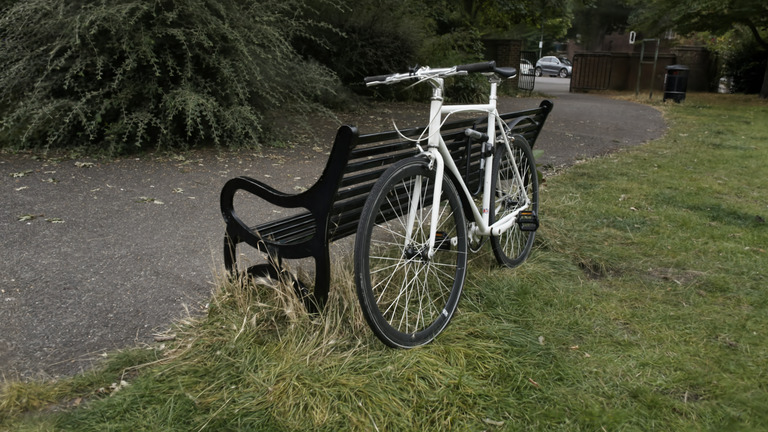
\includegraphics[width=\linewidth]{images/renders/bicycle_rgb_52.jpg}
  \end{subfigure}
  \hfill
  \begin{subfigure}{0.31\linewidth}
  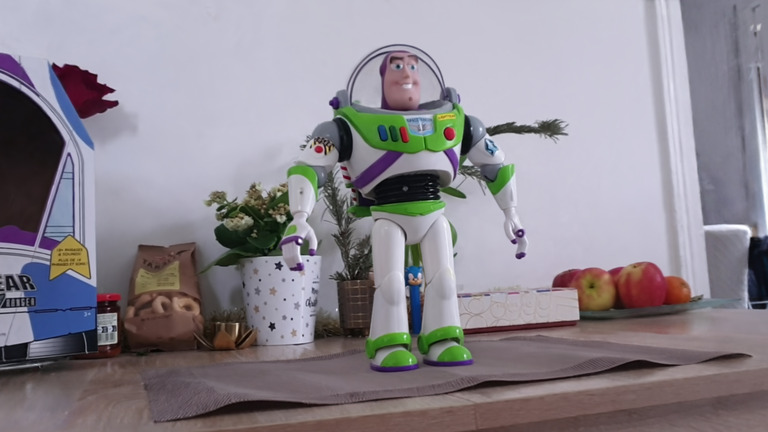
\includegraphics[width=\linewidth]{images/renders/buzz1_rgb_49.jpg}
  \end{subfigure}
  \hfill
  \begin{subfigure}{0.31\linewidth}
  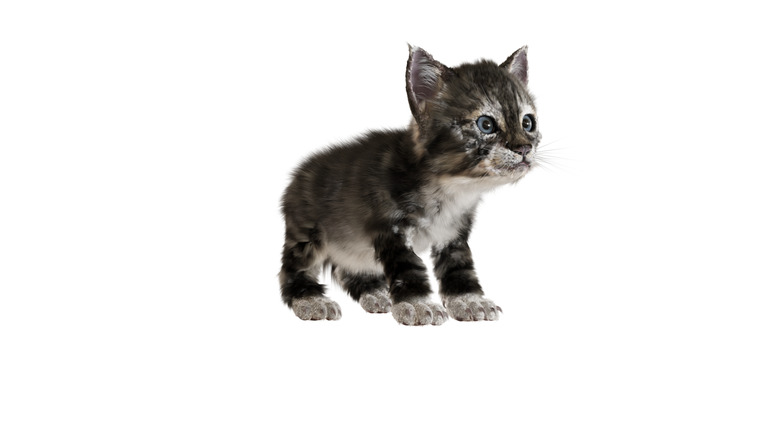
\includegraphics[width=\linewidth]{images/renders/kitten_rgb_42.jpg}
  \end{subfigure}\\
  {\small (a)~Rendering three different scenes with Frosting: \textit{Bicycle}, \textit{Buzz}, and \textit{Kitten}.}\\
  %
  \begin{subfigure}{0.49\linewidth}
  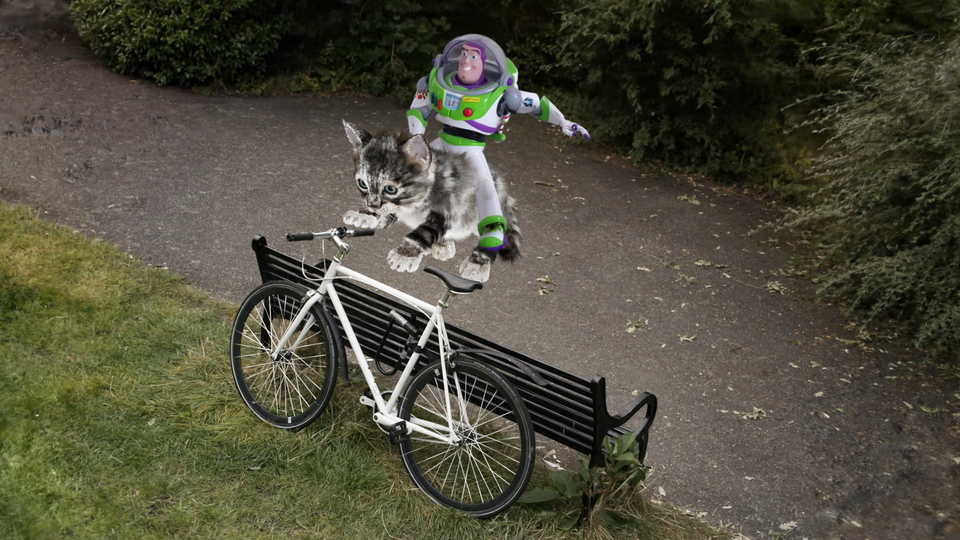
\includegraphics[width=\linewidth]{images/composition/buzz_riding_cat/0_0.png}
  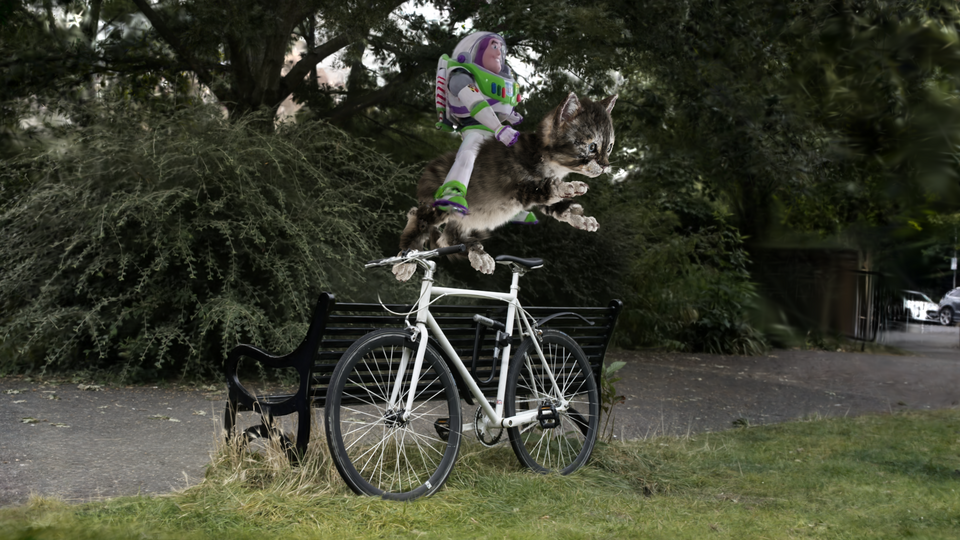
\includegraphics[width=\linewidth]{images/composition/buzz_riding_cat/0_3.png}
  \end{subfigure}
  \hfill
  \begin{subfigure}{0.49\linewidth}
  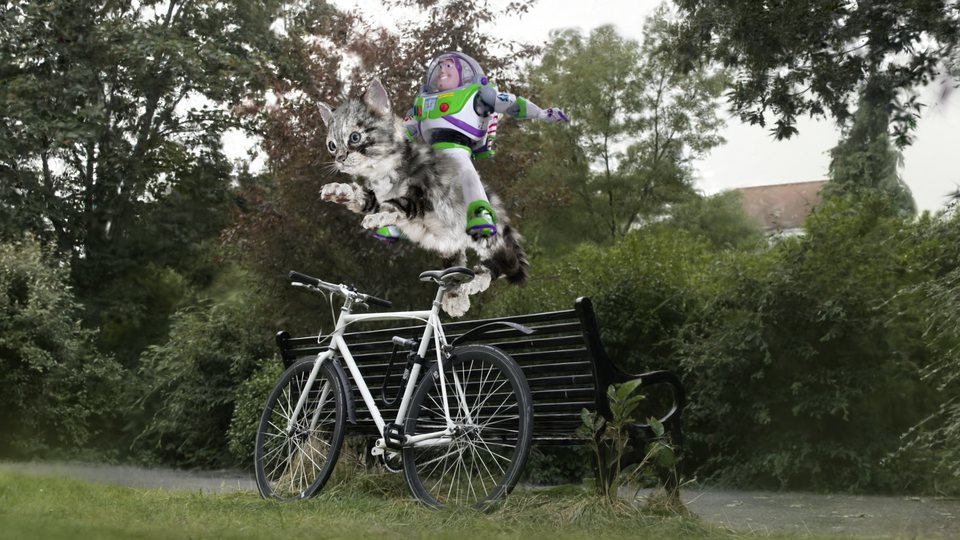
\includegraphics[width=\linewidth]{images/composition/buzz_riding_cat/0_1.png}
  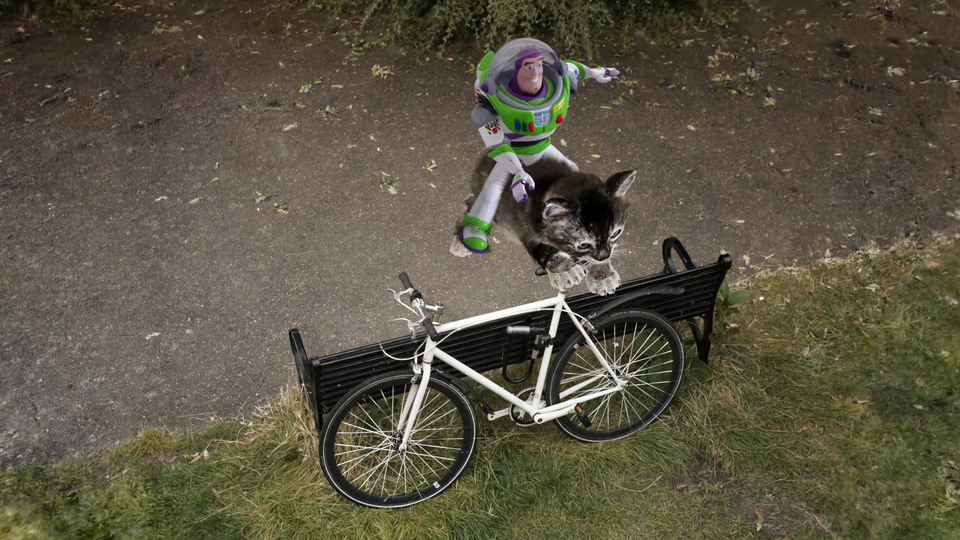
\includegraphics[width=\linewidth]{images/composition/buzz_riding_cat/0_2.png}
  \end{subfigure}
  {\small (b)~Composition: \textit{Buzz is riding a giant kitten jumping over a bench.}}\\
  %
  \begin{subfigure}{0.49\linewidth}
 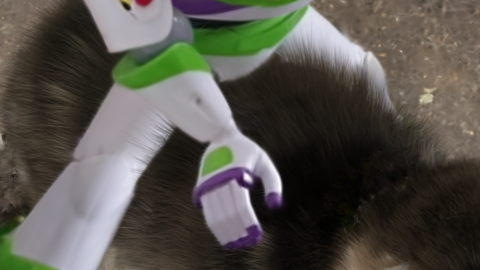
\includegraphics[width=0.49\linewidth]{images/composition/buzz_riding_cat/closeup_1.png}
 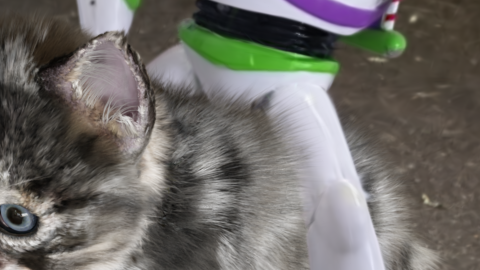
\includegraphics[width=0.49\linewidth]{images/composition/buzz_riding_cat/closeup_2.png}
 \caption*{(c) Fuzzy details rendered with Frosting - occlusions are correctly rendered}
  \end{subfigure}
  %
  \hfill
  %
  \begin{subfigure}{0.49\linewidth}
  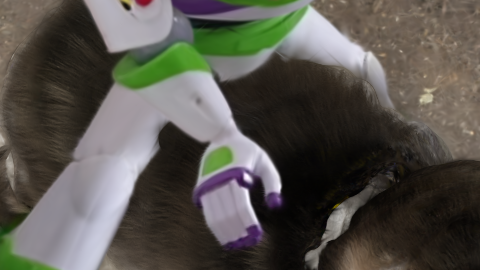
\includegraphics[width=0.49\linewidth]{images/composition/buzz_riding_cat/closeup_1_flat.png}
 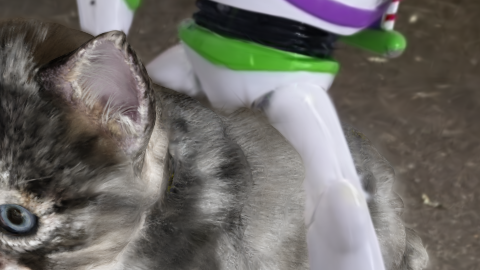
\includegraphics[width=0.49\linewidth]{images/composition/buzz_riding_cat/closeup_2_flat.png}
  \caption*{(d) Rendering with SuGaR~\cite{guedon2023sugar} - the fur does not occlude the legs correctly}
  \end{subfigure}
  %
  \caption{
  % original caption
  % \textbf{Complex scene composition with Frosting.} Frosting has editing capabilities similar to surface-based methods like SuGaR~\cite{guedon2023sugar}, but reaches better performance for rendering complex volumetric effects such as fuzzy materials. In this example, we were able to animate both Buzz and the kitten, changing their original pose (a) while preserving high-quality rendering (b): Contrary to SuGaR, very fine and fuzzy details such as the kitten's hair can be seen covering Buzz's legs in a realistic way (c).
  % final caption
  We propose to represent surfaces by a mesh covered with a ``Frosting'' layer of varying thickness and made of 3D Gaussians. This representation captures both complex volumetric effects created by fuzzy materials such as the cat's hair or grass as well as flat surfaces. 
  Built from RGB images only, it can be rendered in real-time and animated using traditional animation tools.
  In the example above, we were able to animate both Buzz and the kitten, changing their original pose (a) while preserving high-quality rendering (b): Contrary to SuGaR, very fine and fuzzy details such as the kitten's hair can be seen covering Buzz's legs in a realistic way (c).
  }
  \label{fig:sugar-comparison}
\end{figure}
\begin{figure}[h]
  \centering
  
  
   \begin{subfigure}{0.49\linewidth}
  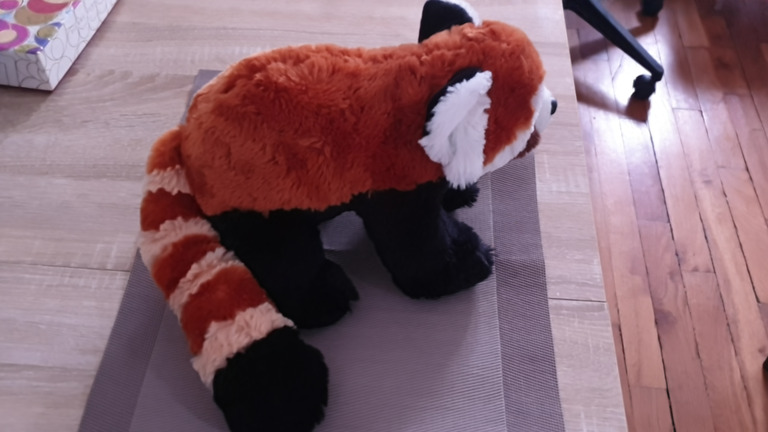
\includegraphics[width=0.99\linewidth]{images/renders/panda1_rgb_166.jpg}
  \caption{Rendering}
  \end{subfigure}
  \hfill
  \begin{subfigure}{0.49\linewidth}
  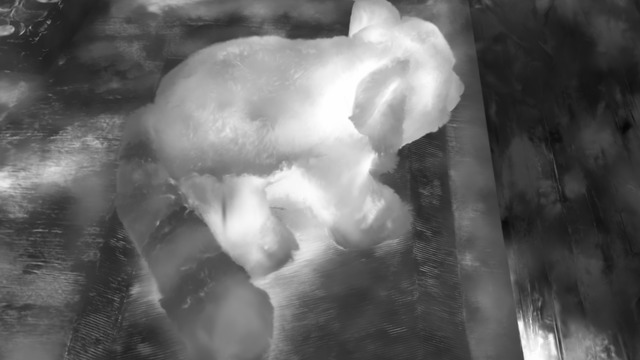
\includegraphics[width=0.99\linewidth]{images/frosting_size/panda1_size_166.jpg}
  \caption{Thickness of the Frosting layer}
  \end{subfigure}
  
  % 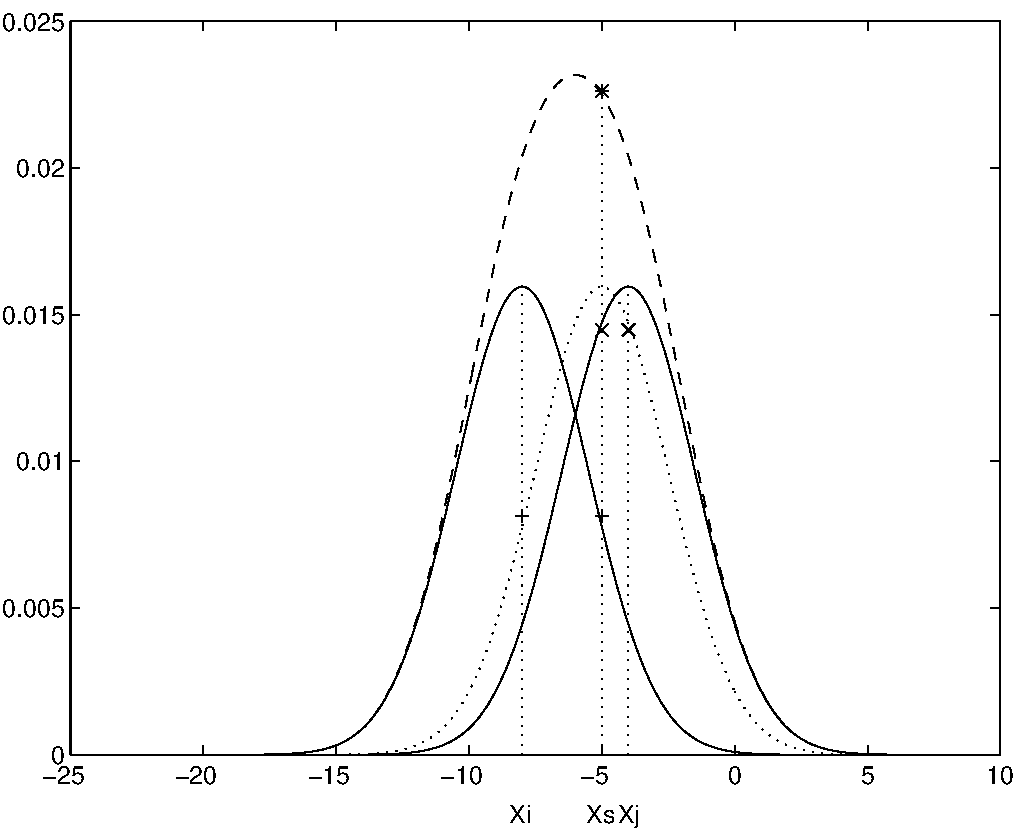
\includegraphics[height=6.5cm]{eijkel2}
  % \fbox{\rule{0pt}{2in} \rule{.9\linewidth}{0pt}}
  \caption{
  % We propose to represent surfaces by a mesh covered with a ``frosting'' layer of varying thickness and made of 3D Gaussians. This representation captures both complex volumetric effects created by fuzzy materials such as the cat's hair as well as flat surfaces. It can be rendered in real-time and animated using traditional animation tools as shown in the video provided as supplementary material. We also propose a method to build this representation from color images and capture fine details as seen in the rendered image and the normal map.
  \textbf{Visualization of the thickness of the Frosting layer on an example.} A thicker layer is shown with a brighter value. Our method automatically builds a thick Frosting layer for fuzzy areas  such as the fur of the red panda plush, and a thin Frosting layer for flat surfaces such as the table or the floor. Adapting the thickness of the Frosting layer allows for allocating more Gaussians in areas where more volumetric rendering is necessary near the surface, resulting in an efficient distribution of Gaussians in the scene. As we demonstrate in the paper, using an adaptive thickness results in higher performance than using a predefined constant thickness, and reduces artifacts when animating the mesh.}
  \label{fig:teaser}
\end{figure}
We propose Gaussian Frosting, a novel mesh-based representation for high-quality rendering and editing of complex 3D effects in real-time. Our approach builds on the recent 3D Gaussian Splatting framework, which optimizes a set of 3D Gaussians to approximate a radiance field from images. We propose first extracting a base mesh from Gaussians during optimization, then building and refining an adaptive layer of Gaussians with a variable thickness around the mesh to better capture the fine details and volumetric effects near the surface, such as hair or grass. We call this layer Gaussian Frosting, as it resembles a coating of frosting on a cake. The fuzzier the material, the thicker the frosting. We also introduce a parameterization of the Gaussians to enforce them to stay inside the frosting layer and automatically adjust their parameters when deforming, rescaling, editing or animating the mesh. Our representation allows for efficient rendering using Gaussian splatting, as well as editing and animation by modifying the base mesh. We demonstrate the effectiveness of our method on various synthetic and real scenes, and show that it outperforms existing surface-based approaches. We will release our code and a web-based viewer as additional contributions.
\keywords{Gaussian Splatting \and Mesh \and Differentiable rendering}
  
\end{abstract}

\vspace{1cm}
\section{Introduction}
\label{sec:intro}

\begin{figure*}[t]
\centering
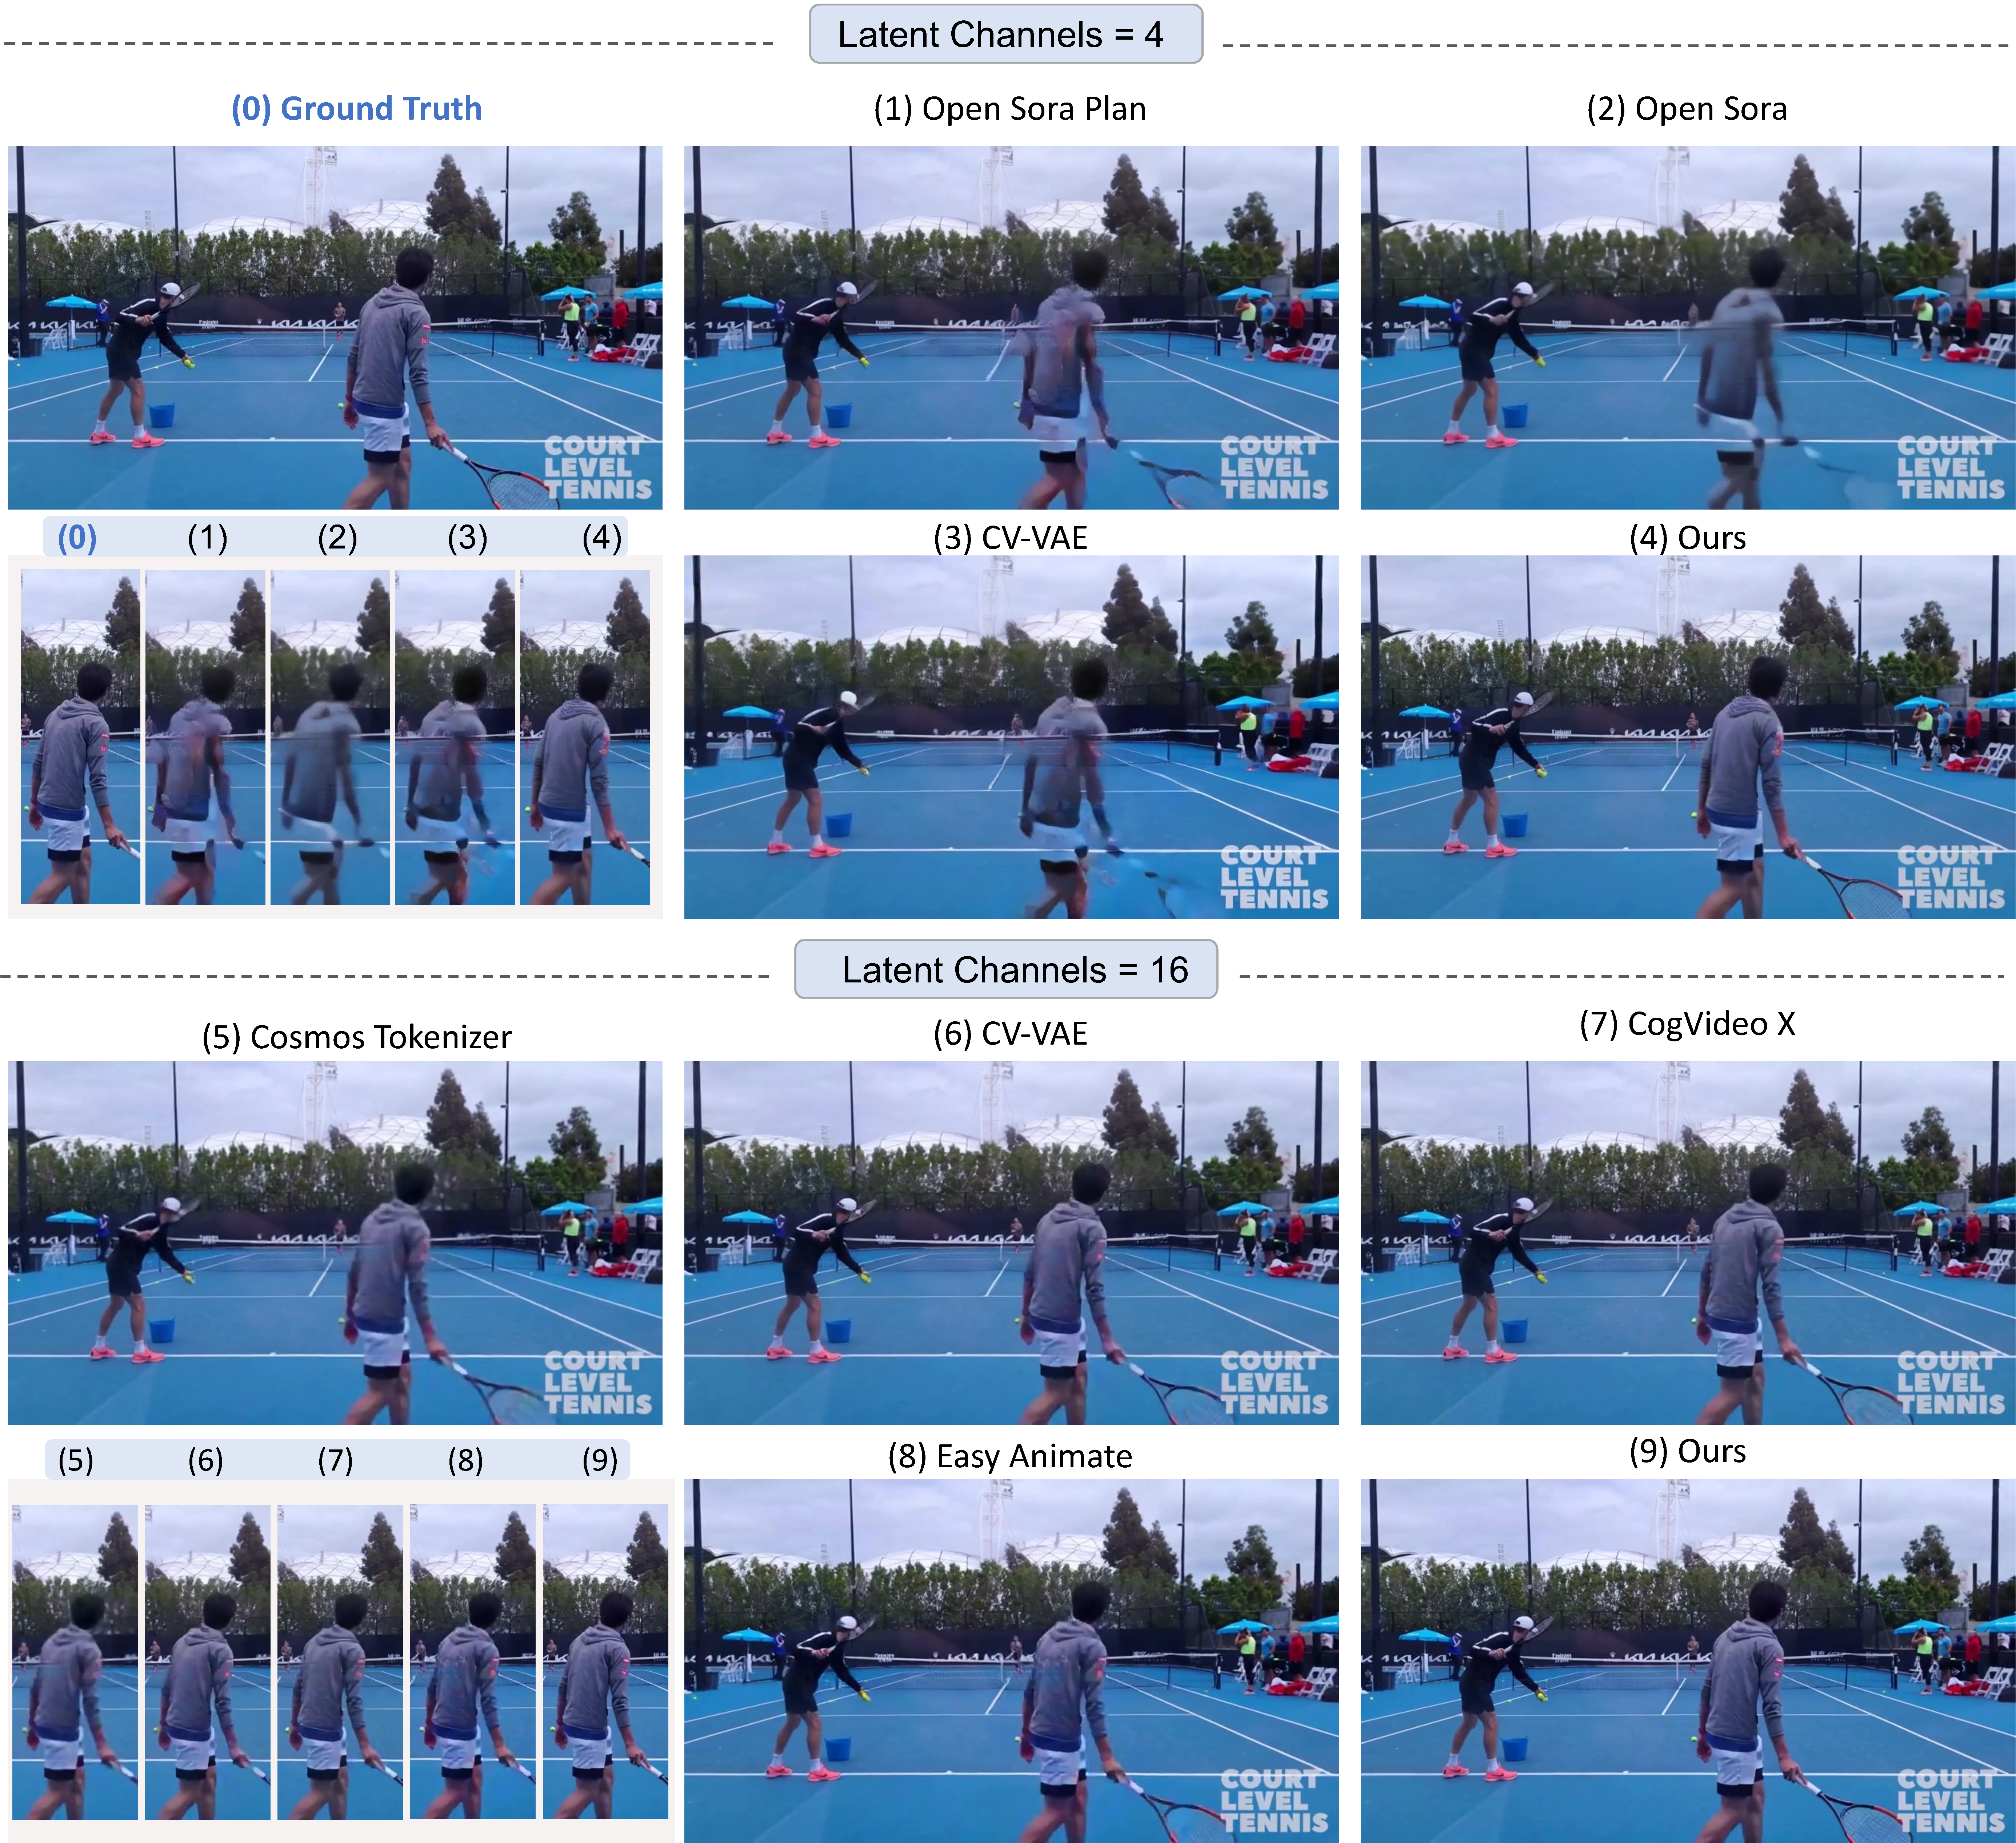
\includegraphics[width=1.0\textwidth]{images/fig1-4and16.pdf}
\caption{
Our reconstruction results compared with a line of three recent strong baseline approaches. 
The ground truth frame is (0). Our model significantly outperforms previous methods, especially under large motion scenarios such as people doing sports.
}
\label{fig:teaser}
\vspace{-3mm}
\end{figure*}



Given the significant attention in the field of video generation, Latent Video Diffusion Models (LVDMs)~\cite{blattmann2023stable, blattmann2023align, he-lvdm, zhou2022magicvideo, he-videocrafter1} have emerged as a popular framework. They have been successfully applied to powerful text-to-video models such as Sora~\cite{videoworldsimulators2024}, VideoCrafter~\cite{he-videocrafter1, chen2024videocrafter2overcomingdatalimitations}, and CogVideoX~\cite{yang2024cogvideox}.
Different from directly generating video pixels, LVDMs generate latent video representations in a compact latent space. This is achieved by first training a Video VAE to encode videos into this latent space.
%
Thus, Video VAE, as a key and fundamental component of LVDMs, has attracted great attention recently.
%
An effective Video VAE can help to reduce the training costs of video diffusion models while improving the final quality of the generated videos.
%
Initially, a series of studies adopt the image VAE from Stable Diffusion~\cite{rombach2022high} for video generation tasks, including AnimateDiff~\cite{guoanimatediff}, MagicVideo~\cite{zhou2022magicvideo}, VideoCrafter1~\cite{he-videocrafter1}, and VideoCrafter2~\cite{chen2024videocrafter2overcomingdatalimitations}. 
%
However, directly adopting an image VAE and compressing video on a frame-by-frame basis leads to temporal flickering due to the lack of temporal correlation. Additionally, the information redundancy along the temporal dimension is not reduced, leading to low training efficiency for subsequent latent video diffusion models.
%
From the introduction of Sora, which compresses videos both temporally and spatially through a Video VAE, a series of studies have emerged that aim to replicate Sora and train their own Video VAEs, including Open Sora~\cite{opensora}, Open Sora Plan~\cite{pku_yuan_lab_and_tuzhan_ai_etc_2024_10948109}, CV-VAE~\cite{zhao2024cv}, CogVideoX~\cite{yang2024cogvideox}, EasyAnimate~\cite{xu2024easyanimatehighperformancelongvideo}, and Cosmos Tokenizer~\cite{cosmos_token}.
%
However, the performance of the current video VAE suffers from many problems, including motion ghost, low-level temporal flickering, blurring (faces, hands, edges, texts), and motion stuttering (lack of correct temporal transition).
% as shown in Fig.~\ref{fig:teaser}.


In this work, we propose a novel cross-modal Video VAE with better spatial and temporal modeling ability in order to solve the aforementioned challenge problems and obtain a robust and high-quality Video VAE.
%
First, we examine different designs for spatial and temporal compression, including simultaneous spatial-temporal (ST) compression and sequential ST compression. 
%
We observed that simultaneous ST compression achieves better low-level temporal smoothness and texture stability, while sequential ST compression achieves better motion recovery, particularly in scenarios of large motion.
%
Thus, we propose a novel architecture that integrates the advantages of both methods and enables effective video detail and motion reconstruction.

Second, we observed that the normally used datasets for text-to-video generation contain text-video pairs. 
Also, during decoding, a text description exists as it serves as the input in the first stage, \textit{i.e.}, the video latent generation stage.
%
To this end, we integrate the text information into the encoding and decoding procedure and propose the first Cross-modal Video VAE.
%
We carefully study how text guidance can be integrated into the spatiotemporal backbone and the mechanism of spatial and temporal semantic guidance. 

In addition, our cross-modal video VAE supports image-video joint training.
To achieve this, we design our network with a fully spatiotemporal factorized architecture, and we feed image and video batches alternately to the network. 
%
During image batches, the data only forwards the spatial part of the network, with the temporal modules being skipped. During video batches, the video forwards both spatial and temporal modules. We also demonstrate that image joint training is crucial for training a video VAE.
%
In summary, our contributions are as follows:
\begin{itemize}
    \item We propose an effective and robust Video VAE, conduct extensive experiments, and achieve the state-of-the-art.
    \item We propose an optimal spatiotemporal modeling approach for Video VAE.
    \item We propose the first cross-modal video VAE that leverages the information from other modalities, i.e., text descriptions, to the best of our knowledge.
    \item Our video VAE is designed and trained to be versatile to conduct both image and video compression. 
\end{itemize}


\begin{figure}[ht]
  \centering
  \begin{subfigure}{0.14\linewidth}
 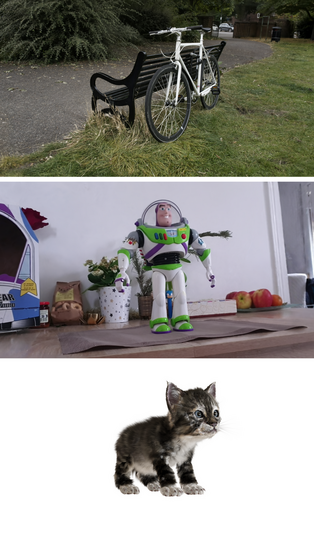
\includegraphics[width=\linewidth]{images/composition/buzz_riding_cat/scenes.png}
 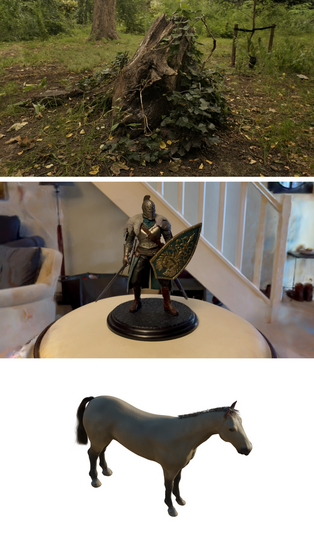
\includegraphics[width=\linewidth]{images/composition/knight_and_horse/scenes.png}
 \caption{Scenes}
  \end{subfigure}
  %
  \hfill
  %
  \begin{subfigure}{0.42\linewidth}
 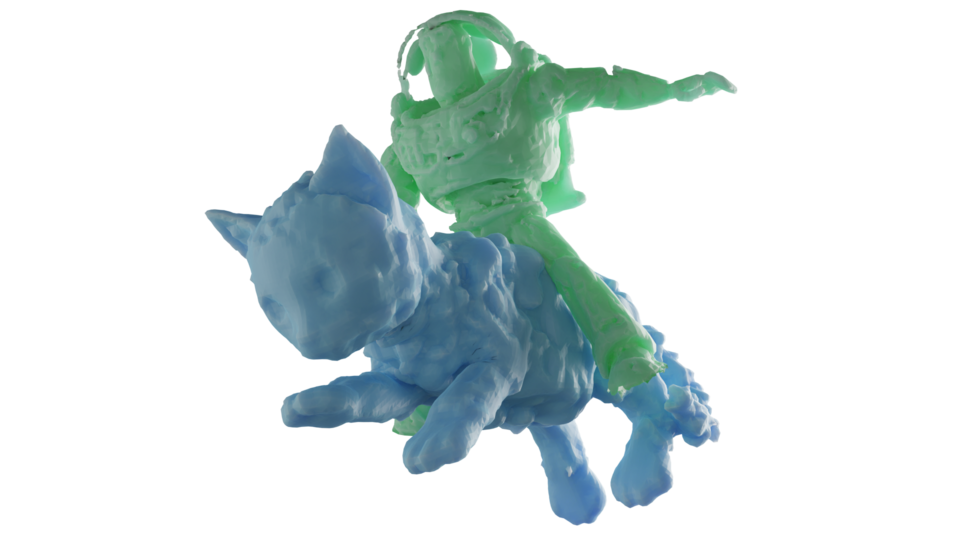
\includegraphics[width=\linewidth]{images/composition/buzz_riding_cat/mesh.png}
 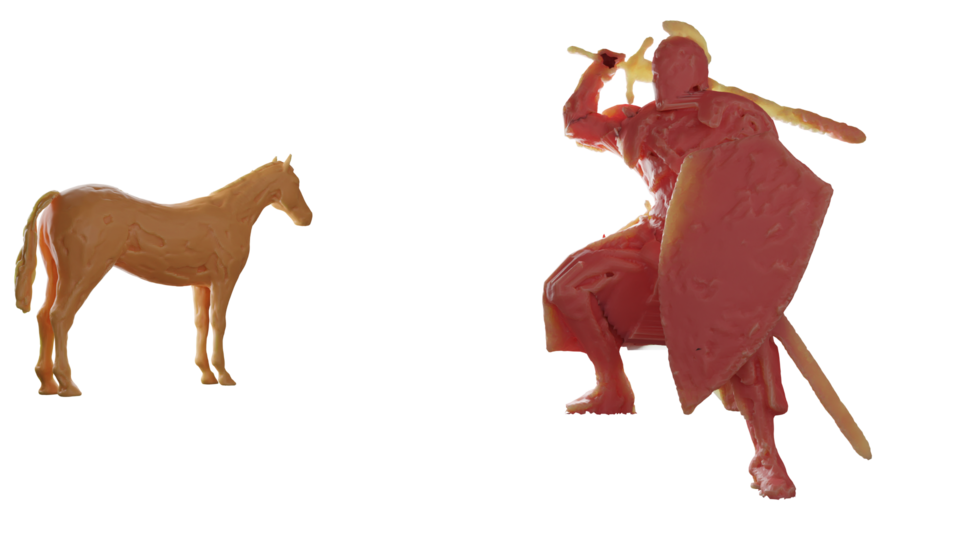
\includegraphics[width=\linewidth]{images/composition/knight_and_horse/mesh.png}
  \caption{Posing foreground meshes}
  \end{subfigure}
  %
  \hfill
  \begin{subfigure}{0.42\linewidth}
 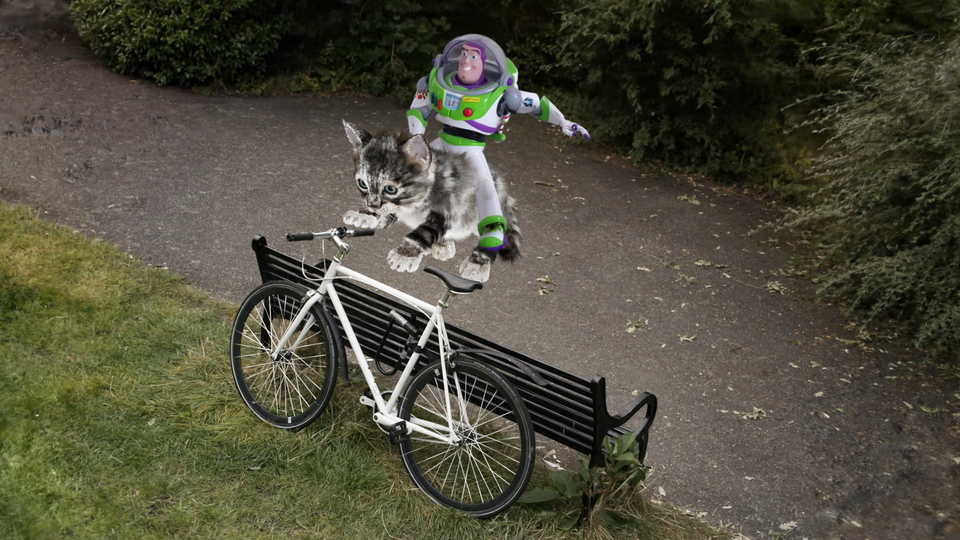
\includegraphics[width=\linewidth]{images/composition/buzz_riding_cat/0_0.png}
 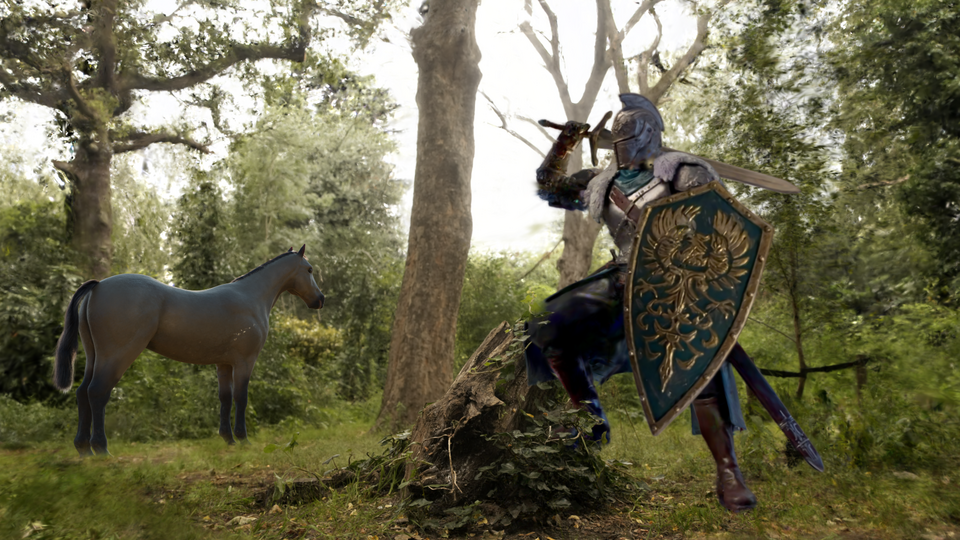
\includegraphics[width=\linewidth]{images/composition/knight_and_horse/0_1.png}
  \caption{Rendering composition}
  \end{subfigure}
  %
  \caption{
  \textbf{Scene composition.} Using mesh editing tools in Blender, we were able to combine various elements from multiple scenes (a) to build a whole new scene (c). We also changed the pose of the characters by using the rigging tool in Blender (b). Similarly to surface-based methods like SuGaR~\cite{guedon2023sugar}, Frosting can be used for editing and compositing scenes, but allows for better rendering of complex volumetric effects and fuzzy materials, such as hair or grass.
  }
  \label{fig:scene-composition}
\end{figure}

\section{Related Work}

The goal of image-based rendering (IBR) is to create a representation of a scene from a given set of images in order to generate new images of the scene. Different types of scene representations have been proposed, ranging from explicit and editable ones like triangle meshes or point clouds, to implicit or non-editable ones like voxel grids, multiplane images, or neural implicit functions. 

\noindent
\textbf{Volumetric IBR methods.} A recent breakthrough in IBR is Neural Radiance Fields (NeRF)~\cite{mildenhall2020nerf}, which uses a multilayer perceptron (MLP) to model a continuous volumetric function of density and color. NeRF can render novel views with high quality and view-dependent effects, by using volumetric ray tracing. However, NeRF is slow and memory hungry. 
%
Several works have tried to improve NeRF’s efficiency and training speed by using discretized volumetric representations like voxel grids and hash tables to store learnable features that act as inputs for a much smaller MLP~\cite{chen-eccv-2022-tensorf, karnewar2022relu, mueller2022instantngp, sun2022direct, yu_and_fridovichkeil2021plenoxels}, or to improve rendering performance by using hierarchical sampling strategies~\cite{barron2022mipnerf360,hedman2021snerg,reiser2021kilonerf,yu2021plenoctrees}. Other works have also proposed to modify NeRF's representation of radiance and include an explicit lighting model to increase the rendering quality for scenes with specular materials~\cite{verbin2022ref, boss2021nerd, kuang2022neroic, srinivasan2021nerv, zhang2021physg}. 
%
However, most volumetric methods rely on implicit representations that are not suited to editing compared to triangle meshes, for which most standard graphics hardware and software are tailored.

\noindent
\textbf{Surface-based IBR methods.} Triangle meshes have been a popular 3D representation for generating novel views of scenes~\cite{wood:2000:slf,buehler2001unstructured,hedman-2018-deepblending} after Structure-from-motion (SfM)~\cite{snavely-2006-structure-from-motion} and multi-view stereo (MVS)~\cite{goesele-2007-multiviewstereo} have enabled 3D reconstruction of surfaces. 
%
Deep-learning-based mesh representations~\cite{riegler2020free,riegler2021stable} have also been used for improving view synthesis using explicit surface meshes; However, even though mesh-based methods allow for very efficient rendering, they have trouble capturing complex and very fine geometry as well as fuzzy materials.

\noindent
\textbf{Hybrid IBR methods.} Some methods use a hybrid volumetric representation to recover surface meshes that are suitable for downstream graphics applications while efficiently modeling view-dependent appearance. 
%
Specifically, some works optimize a Neural Radiance Field in which the density is replaced by an implicit signed distance function (SDF), which provides a stronger regularization on the underlying geometry~\cite{oechsle2021unisurf,yariv2021volsdf,wang2021neus,li-cvpr2023-neuralangelo,darmon-2022-warp,bao-2022-neumesh}. However, most of these methods are not aimed at real-time rendering.
To mitigate this issue, other approaches greatly accelerate rendering by ``baking'' the rendering computation into the extracted mesh after optimization with a dedicated view-dependent appearance model~\cite{chen2022mobilenerf,yariv-2023-bakedsdf,reiser2024binaryopacitygrid}. 
%
Even though these surface-based methods encode the surface using a volumetric function represented by an MLP during optimization, they struggle in capturing fine details or fuzzy materials compared to volumetric methods.

Adaptive Shells~\cite{wang-siggraphasia2023-adaptive-shells} is a recent method that achieves a significant improvement in rendering quality by using a true hybrid surface-volumetric approach that restricts the volumetric rendering of NeRFs to a thin layer around the object. This layer is bounded by two explicit meshes, which are extracted after optimizing an SDF-based radiance field. The layer’s variable thickness also improves the rendering quality compared to a single flat mesh. This method combines the high-quality rendering of a full volumetric approach with the editability of a surface-based approach by manipulating the two meshes that define the layer. However, Adaptive Shells depends on a neural SDF~\cite{wang2021neus}, which has some limitations in its ability to reconstruct precise surfaces, and requires more than 8 hours to optimize a single synthetic scene, which is much longer than the recent Gaussian Splatting methods. 

\noindent
\textbf{Gaussian Splatting.} Gaussian Splatting~\cite{kerbl3Dgaussians} is a new volumetric representation inspired by point cloud-based radiance fields~\cite{kopanas2021point, ruckert2021adop} which is very fast to optimize and allows for real-time rendering with very good quality. One of its greatest strengths is its explicit 3D representation, which enables editing tasks as each Gaussian exists individually and can be easily adjusted in real-time. 
%
Some appearance editing and segmentation methods have been proposed~\cite{chen2023gaussianeditor,huang2023pointn,chungmin-2024-garfield,ye-2023-gaussian_grouping}, but the lack of structure in the point cloud makes it almost impossible for a 3D artist or an animator to easily modify, sculpt or animate the raw representation. The triangle mesh remains the standard 3D structure for these applications.
%
A recent work, SuGaR~\cite{guedon2023sugar}, extends this framework by aligning the Gaussians with the surface and extracting a mesh from them. Gaussians are finally flattened and pinned on the surface of the mesh, which provides a hybrid representation combining the editability of a mesh with the high-quality rendering of Gaussian Splatting. However, SuGaR remains a surface-based representation with limited capacity in reconstructing and rendering fuzzy materials and volumetric effects, resulting in a decrease in performance compared to vanilla Gaussian Splatting.
\section{3D Gaussian Splatting and Surface Reconstruction}

Our method relies on the original 3D Gaussian Splatting~(3DGS) method~\cite{kerbl3Dgaussians} for initialization and on SuGaR~\cite{guedon2023sugar} to align Gaussians with the surface of the scene and facilitate the extraction of a mesh. We briefly describe 3DGS and SuGaR in this section before describing our method in the next section.


\subsection{3D Gaussian Splatting} 

3DGS represents the scene as a large set of Gaussians. Each Gaussian $g$ is equipped with a mean $\mu_g\in \IR^3$ and a positive-definite covariance matrix $\Sigma_g\in \IR^{3\times 3}$. The covariance matrix is parameterized by a scaling vector $s_g\in\IR^3$ and a quaternion $q_g\in\IR^4$ encoding the rotation of the Gaussian. 

In addition, each Gaussian has a view-dependent radiance represented by an opacity $\alpha_g\in [0,1]$ and a set of spherical harmonics coordinates defining the colors emitted for all directions. To render an image from a given viewpoint, a rasterizer ``splats'' the 3D Gaussians into 2D Gaussians parallel to the image plane and blends the splats depending on their opacity and depth. This rendering is extremely fast, which is one of the advantages of 3DGS over volumetric rendering as in NeRFs for example~\cite{mildenhall2020nerf, mueller2022instantngp, barron2022mipnerf360}.


Gaussian Splatting can be seen as an approximation of the traditional volumetric rendering of radiance fields with the following density function $d$, computed as the sum of the Gaussian values weighted by their alpha-blending coefficients at any 3D point $p\in \IR^3$:
%
 \begin{equation}
    d(p) = \sum_{g} \alpha_g \exp\left(-\frac{1}{2}(p - \mu_g)^T \Sigma^{-1}_g (p - \mu_g)\right) \> .
    \label{eq:gaussian_splatting_density}
\end{equation}

We initialize our Gaussian Frosting method using a vanilla 3DGS optimization: Gaussians are initialized using the point cloud produced by an SfM~\cite{snavely-2006-structure-from-motion} algorithm like COLMAP~\cite{schoenberger2016mvs,schoenberger2016sfm}, required to compute camera poses. The Gaussians' parameters (3D means, scaling vectors, quaternions, opacities, and spherical harmonics coordinates) are then optimized to make the renderings match the ground truth images of the scene, using a rendering loss that only consists in a combination of a pixel-wise L1 distance and a more structural D-SSIM term. 


\subsection{SuGaR Mesh Extraction} 

Vanilla 3DGS does not have regularization explicitly encouraging Gaussians to align with the true surface of the scene. Our Gaussian Frosting representation relies on a mesh that approximates this surface, in order to be editable by traditional tools. To obtain this mesh, we rely on the method proposed in SuGaR~\cite{guedon2023sugar}, which we improve by automatically selecting a critical hyperparameter.

SuGaR proposes a regularization term encouraging the alignment of the 3D Gaussians with the true surface of the scene during the optimization of Gaussian Splatting, as well as a mesh extraction method. After enforcing the regularization, the optimization provides Gaussians that are mostly aligned with the surface albeit not perfectly: We noticed that in practice, a large discrepancy between the regularized Gaussians and the extracted mesh indicates the presence of fuzzy materials or surfaces that require volumetric rendering. We thus exploit this discrepancy as a cue to evaluate where the Frosting should be thicker.

\begin{figure}[tb]
  \centering
  % 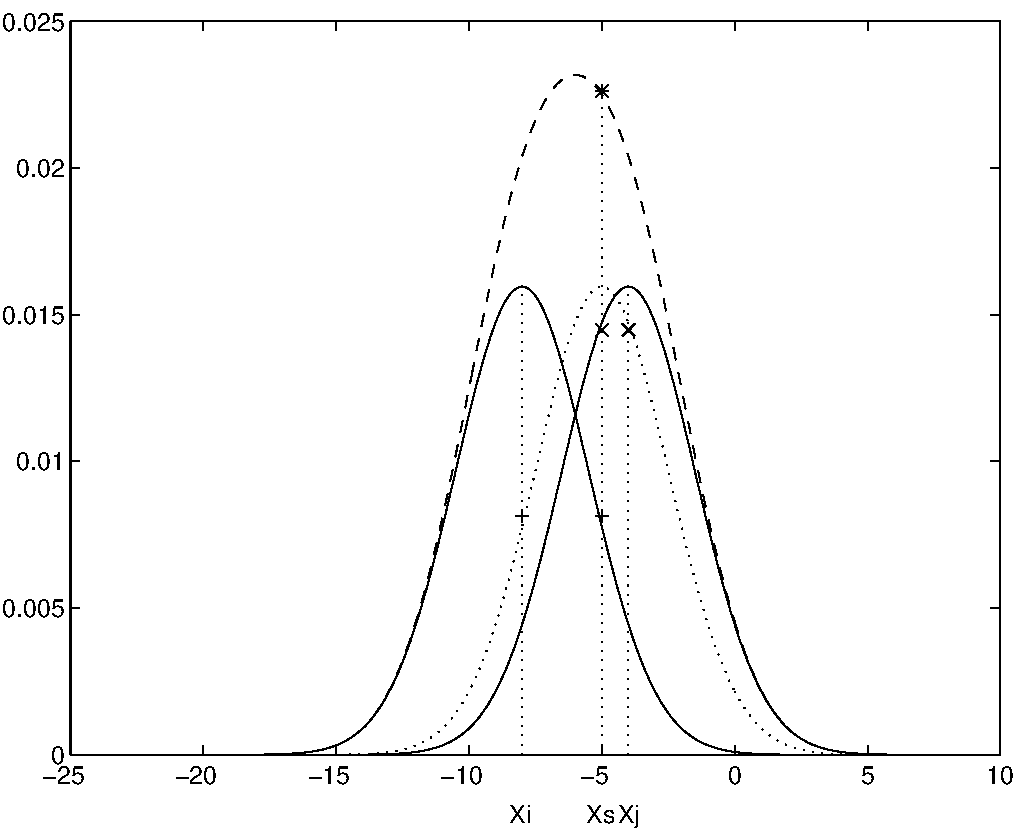
\includegraphics[height=6.5cm]{eijkel2}
  % \fbox{\rule{0pt}{0.8in} \rule{.95\linewidth}{0pt}}
  %\includesvg[inkscapelatex=false, width = 1\linewidth]{images/pipeline_frosting_largefont}
  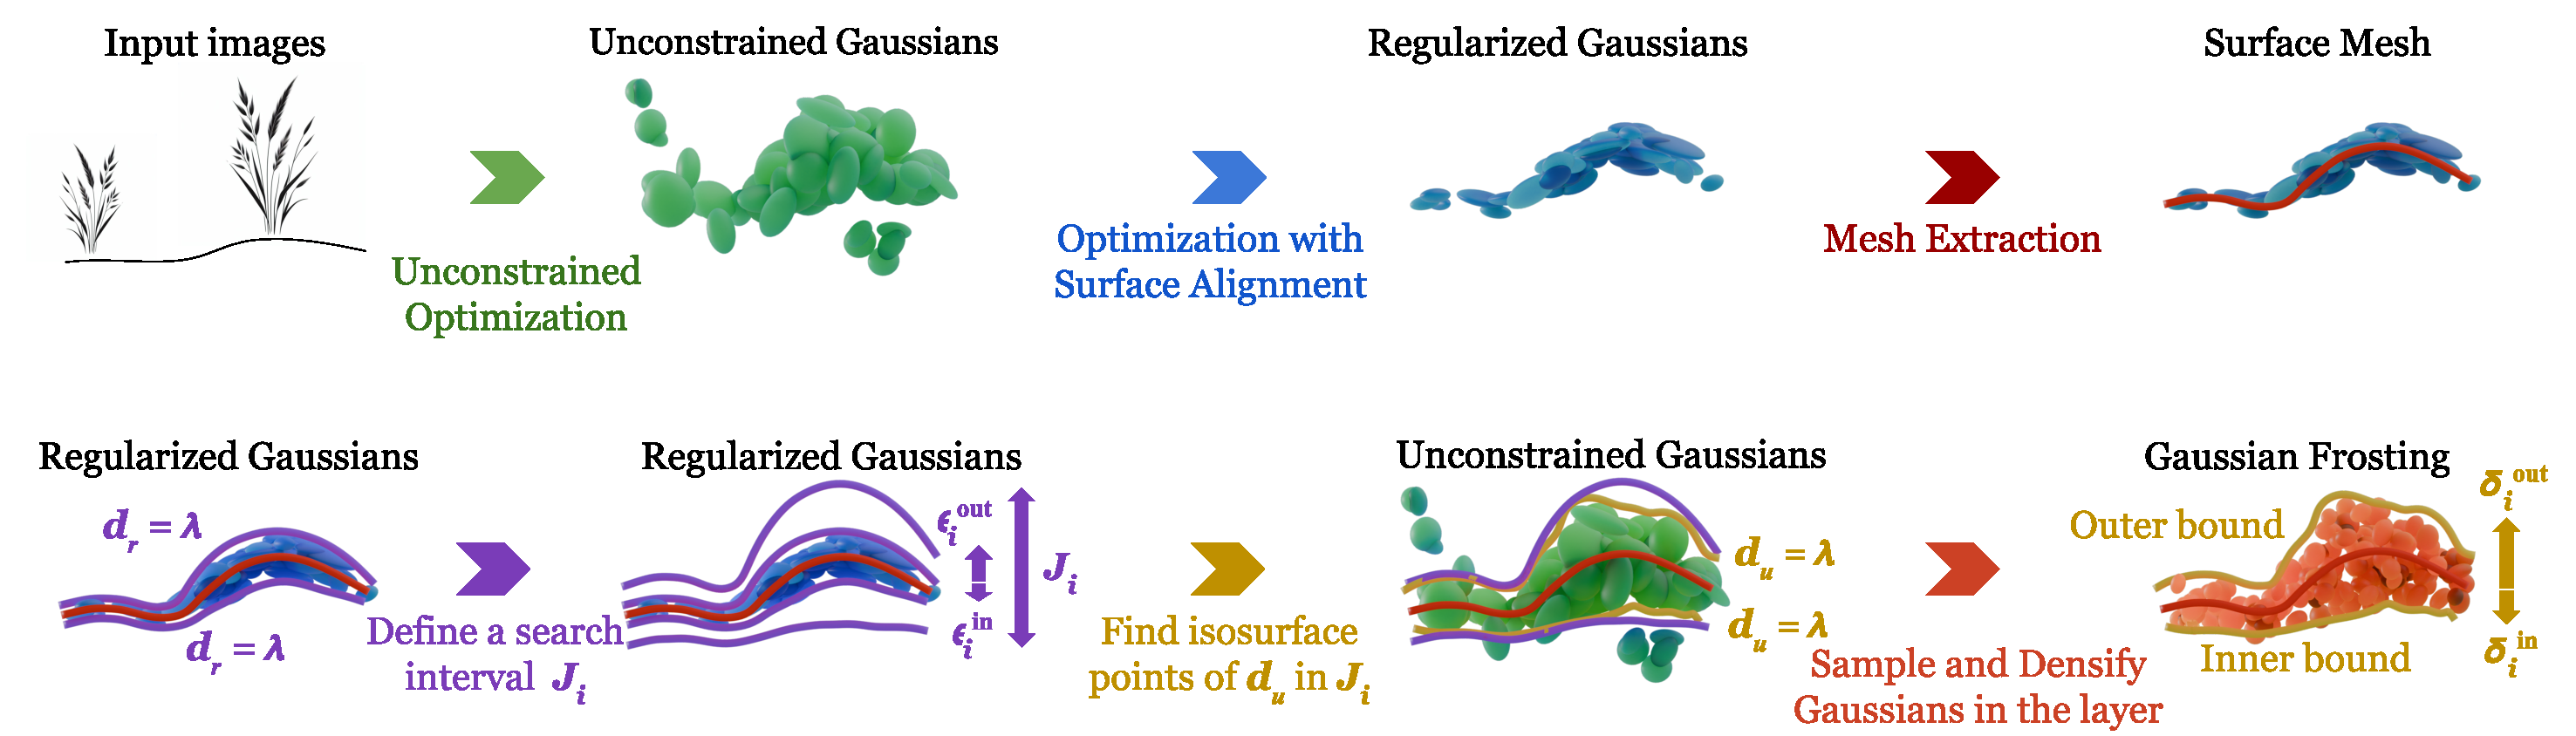
\includegraphics[width=\linewidth]{images/pipeline_frosting_largefont.pdf}
  \caption{
  \textbf{Creating a Layer of Gaussian Frosting.} To build our proposed Frosting representation, we start by optimizing a Gaussian Splatting representation using a rendering loss without any additional constraint, to let Gaussians position themselves. We refer to these Gaussians as \emph{unconstrained}. We then regularize these Gaussians to enforce their alignement with the surface, and extract a mesh that will serve as a basis for the Frosting. Next, we use the misalignment of surface-aligned Gaussians to identify areas where more volumetric rendering is needed, and we build search intervals $J_i$ around the mesh's vertices $\vec{v_i}$. Finally, we use the density function of the unconstrained Gaussians to refine the intervals, resulting in a Frosting layer. We finally sample a novel, densified set of Gaussians inside the layer.
}
  \label{fig:frosting-pipeline}
\end{figure}

\section{Creating a Frosting Layer from Images}

In this section, we describe our Gaussian Frosting creation method: 
First, we extract an editable surface with optimal resolution using SuGaR. We then detail how we use this surface-based model to go back to a volumetric but editable representation built around the mesh. This representation adapts to the complexity of the scene and its need for more volumetric effects. Finally, we describe how we parameterize and refine this representation. An overview is provided Figure~\ref{fig:frosting-pipeline}.

\subsection{Forward Process: From Volume to Surface}
\label{subsec:forward-process}

We start by optimizing an unconstrained Gaussian Splatting representation for a short period of time to let Gaussians position themselves. We will refer to such Gaussians as \emph{unconstrained}. We save these Gaussians aside, and apply the regularization term from SuGaR to enforce the alignment of the Gaussians with the real surface. We will refer to these Gaussians as \emph{regularized}.

Once we obtain the regularized Gaussians, we extract a surface mesh from the Gaussian Splatting representation. This surface mesh serves as a basis for our representation. Like SuGaR~\cite{guedon2023sugar}, we then sample points on the visible level set of the Gaussian splatting density function, and apply Poisson reconstruction. 

In the supplementary material, we describe our technique to automatically estimate a good value for a critical hyperparameter used by Poisson reconstruction, namely the octree depth $D$. As we will show in the Experiments section, selecting the right value for $D$ when applying Poisson reconstruction can drastically improve both the quality of the mesh and the rendering performance of our model. Figure~\ref{fig:mesh-comparison} illustrates this point.


\begin{figure}[tb]
  \centering
  \begin{subfigure}{0.19\linewidth}
  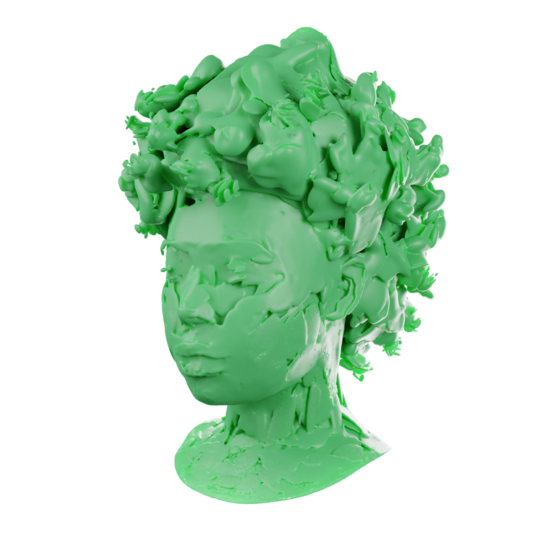
\includegraphics[width=\linewidth]{images/meshes/khady_sugar.png}
  \end{subfigure}
  %
  \hfill
  %
  \begin{subfigure}{0.19\linewidth}
  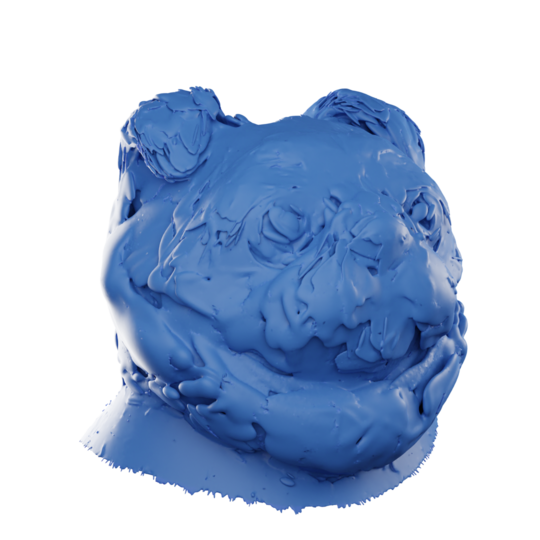
\includegraphics[width=\linewidth]{images/meshes/pug_sugar.png}
  \end{subfigure}
  %
  \hfill
  %
  \begin{subfigure}{0.19\linewidth}
  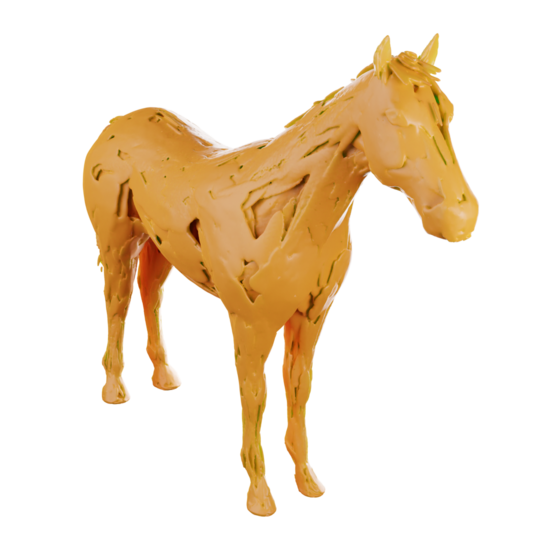
\includegraphics[width=\linewidth]{images/meshes/horse_y_sugar.png}
  \end{subfigure}
  %
  \hfill
  %
  \begin{subfigure}{0.19\linewidth}
  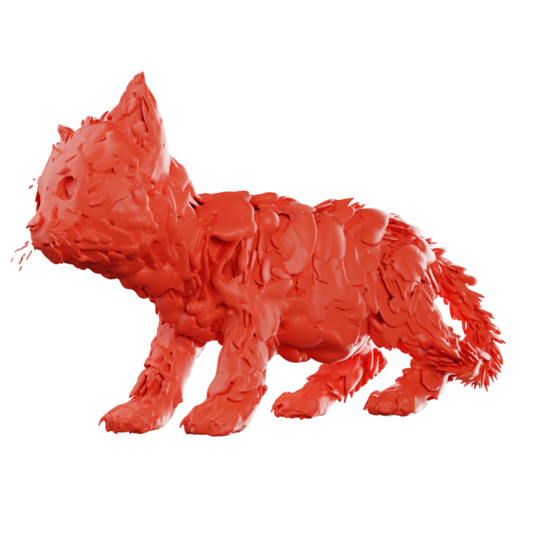
\includegraphics[width=\linewidth]{images/meshes/kitten_sugar.png}
  \end{subfigure}
  %\hfill
  %
  % \begin{subfigure}{0.19\linewidth}
  % \includegraphics[width=\linewidth]{images/meshes/woolly_sugar.png}
  % \end{subfigure}
  %
  %
  \vspace{0.005\linewidth}\\
  {\small (a) Using the predefined, large parameter $D$ as in SuGaR~\cite{guedon2023sugar}} 
  % \vspace{0.01\linewidth}
  \\
  %
  \begin{subfigure}{0.19\linewidth}
  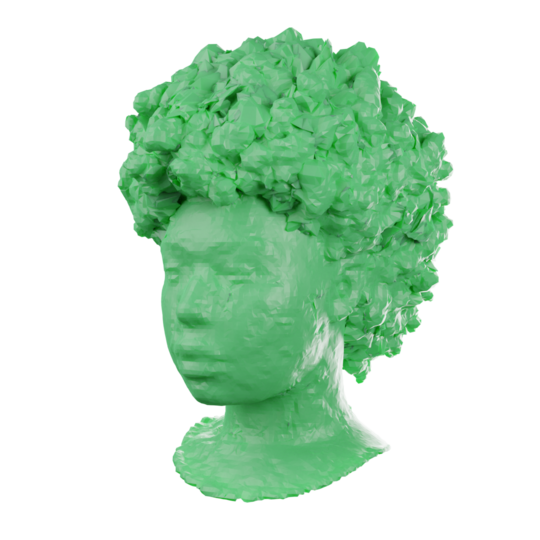
\includegraphics[width=\linewidth]{images/meshes/khady_frosting.png}
  \end{subfigure}
  %
  \hfill
  %
  \begin{subfigure}{0.19\linewidth}
  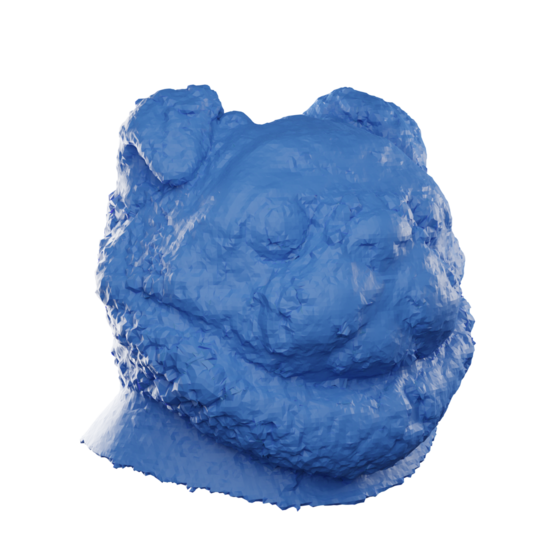
\includegraphics[width=\linewidth]{images/meshes/pug_frosting.png}
  \end{subfigure}
  %
  \hfill
  %
  \begin{subfigure}{0.19\linewidth}
  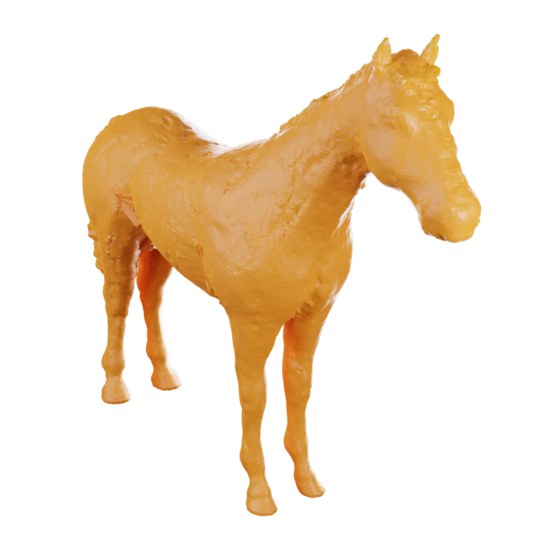
\includegraphics[width=\linewidth]{images/meshes/horse_y_frosting.png}
  \end{subfigure}
  %
  \hfill
  %
  \begin{subfigure}{0.19\linewidth}
  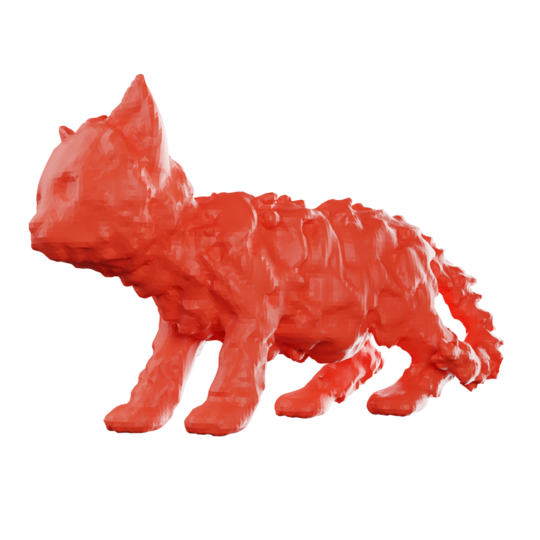
\includegraphics[width=\linewidth]{images/meshes/kitten_frosting.png}
  \end{subfigure}
  %
  % \hfill
  % %
  % \begin{subfigure}{0.19\linewidth}
  % \includegraphics[width=\linewidth]{images/meshes/woolly_frosting.png}
  % \end{subfigure}
  %
  % \vspace{0.005\linewidth}
  \\
  {\small (b) Using our automatically computed $D$ that adapts to the complexity of the 3DGS}
  %
  \caption{
  \textbf{Comparison of meshes extracted by SuGaR from the Shelly dataset without and with our improvement that automatically tunes the octree depth $D$ in Poisson reconstruction depending on the complexity of the scene.}
  Our technique~(bottom) drastically reduces surface artifacts for many scenes, such as the holes and the ellipsoidal bumps on the surface when using the default values from~\cite{guedon2023sugar}~(top).
}
  % \vincentrmk{I would remove the purple thing on the right, the 2 meshes are not very different}
%  \vincentrmk{I removed the wooly thing}
  % Moreover, the outer bound of the frosting layer~(bottom), which is computed using the unconstrained, non-aligned Gaussians, generally provides a refined mesh with better quality than the mesh directly obtained from the isosurface of the aligned Gaussians.
  
  
    % \textbf{Comparison of meshes reconstructed from Gaussian Splatting representations using SuGaR~\cite{guedon2023sugar} and our approach.}
  % Our method to compute automatically optimal hyperparameters for Poisson recontruction~(center) drastically reduces surface artifacts for a lot of scenes, such as the ellipsoidal bumps on the surface when using the default values from~\cite{guedon2023sugar}~(left). Moreover, the outer bound of the frosting layer~(right), which is computed using the unconstrained, non-aligned Gaussians, generally provides a refined mesh with better quality than the mesh directly obtained from the isosurface of the aligned Gaussians.}}
  \label{fig:mesh-comparison}
\end{figure}
% \todo{We also follow SuGaR~\cite{guedon2023sugar} for extracting a base mesh, but we can actually give more details as shown above. Indeed, SuGaR is very elusive on this part; I think it's interesting to understand what Poisson reconstruction provides, that the density functions lacks. Moreover, this part may be important to explain the improvement that I a added, which is a way to automatically compute the optimal octree depth hyperparameter for Poisson reconstruction depending on the configuration of the Gaussians in the scene. This greatly helps to remove "blobs" in the scene without having to tweak the octree depth parameter by hand, so it could be a contribution. Having a well-balanced mesh is important to get a nice frosting.}


\subsection{Backward Process: From Surface to Volume}
\label{sec:shifts}

After extracting a base mesh, we build a Frosting layer with a variable thickness and containing Gaussians around this mesh. We want this layer to be thicker in areas where more volumetric rendering is necessary near the surface, such as fuzzy material like hair or grass for example. On the contrary, this layer should be very thin near the parts of the scene that corresponds to well-defined flat surfaces, such as wood or plastic for example.

\begin{figure}[t]
  \centering
  % \includesvg[inkscapelatex=false, width = 1\linewidth]{images/ray.svg}
  % \includesvg[inkscapelatex=false, width = 1\linewidth]{images/ray.svg}
  % \includesvg[inkscapelatex=false, width = 1\linewidth]{images/ray_w_mesh.svg}
  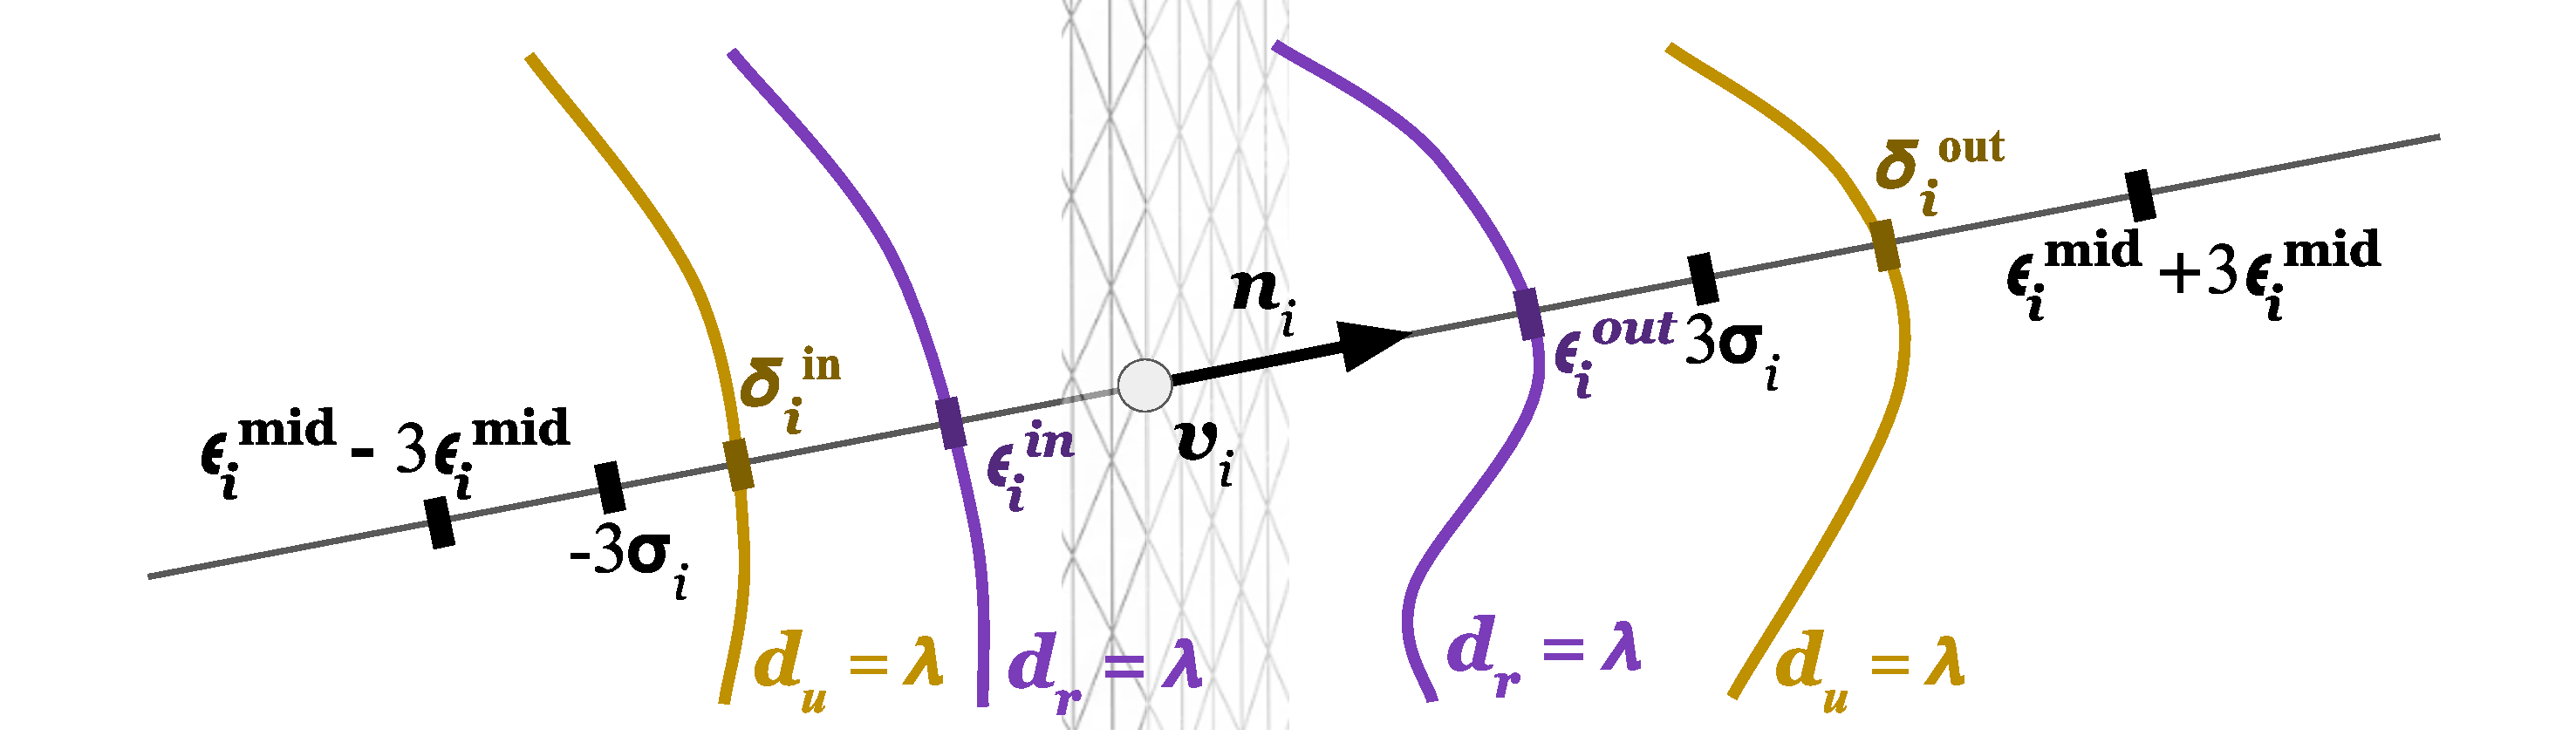
\includegraphics[width=\linewidth]{images/ray_w_mesh.pdf}
  \caption{
  \textbf{How we define the inner and outer bounds of the Frosting layer.} See text in Section~\ref{sec:shifts}.}
  \label{fig:shifts}
\end{figure}


As illustrated in Figure~\ref{fig:shifts}, to define this layer, we introduce two values $\innershift_i$ and $\outershift_i$ for each vertex $\vec{v}_i$ of the extracted base mesh $\calM$. This gives two surfaces with vertices $(\vec{v}_i+\innershift_i \vec{n}_i)_i$ and $(\vec{v}_i+\outershift_i \vec{n}_i)_i$ respectively, where $\vec{n}_i$ is the mesh normal at vertex $\vec{v}_i$. These two surfaces define the inner and outer bounds of the Frosting layer. Note that we do not have to build them explicitly as they directly depend on the base mesh and the $\innershift_i$'s and $\outershift_i$'s.


To find good values for the $\innershift_i$'s and $\outershift_i$'s, we initially tried using directly the unconstrained Gaussians, i.e., the Gaussians obtained before applying the regularization term from SuGaR.  Unfortunately, without regularization, Gaussian Splatting tends to retrieve a thick layer of Gaussians even for ``non-fuzzy'' surfaces, which would result in excessively large values for $\innershift_i$ and $\outershift_i$.  Moreover, the unconstrained Gaussians generally contain many transparent floaters and other outlier Gaussians. Such Gaussians could also bias the shifts toward unnecessarily large values. On the other hand, using only the regularized Gaussians to setup the $\innershift_i$'s and $\outershift_i$'s could miss fuzzy areas since these Gaussians are made flatter by the regularization.


Our solution is thus to consider both the unconstrained and the regularized Gaussians.  More exactly, we estimate the Frosting thickness from the thickness of the unconstrained Gaussians by looking for their isosurfaces, BUT, to make sure we consider the isosurfaces close to the scene surface, we search for the isosurfaces close to the regularized Gaussians: Even under the influence of the regularization term from SuGaR, Gaussians do not align well with the geometry around surfaces with fuzzy details.  As a consequence, the local thickness of the regularized Gaussians is a cue on how fuzzy the material is.


Figure~\ref{fig:shifts}  illustrates what we do to fix the $\innershift_i$'s and $\outershift_i$'s. To restrict the search, we define a first interval $I_i = [-3\sigma_i, 3\sigma_i]$ for each vertex $\vec{v}_i$, where $\sigma_i$ is the standard deviation in the direction of $\vec{n}_i$ of the regularized Gaussian the closest to $\vec{v}_i$. $I_i$ is the confidence interval for the 99.7 confidence level of the 1D Gaussian function of $t$ along the normal. Fuzzy parts result in general in large $I_i$. We could use the $I_i$'s to restrict the search for the isosurfaces of the unconstrained Gaussians. A more reliable search interval $J_i$ is obtained by looking for the isosurfaces of the regularized Gaussians along  $\vec{n}_i$ within $I_i$:
%
\begin{equation}
    \propinnershift_i = \inf ( T ) \text{ , }
    \propoutershift_i = \sup ( T ) \text{ , with }
    T = \left\{ t\in I_i \>\> | \>\> d_r(\vec{v}_i+t\vec{n}_i) \geq \lambda \right\} \> ,
    \label{eq:proposal-shifts}
\end{equation}
%
where $d_r$ is the density function as defined in Eq.~\eqref{eq:gaussian_splatting_density} for the regularized Gaussians.  In practice, we use an isosurface level~$\lambda = 0.01$, i.e., close to zero.
%
We use $ \propinnershift_i$ and $\propoutershift_i$ to define interval $J_i$: $J_i = \left[ \epsilon^\Mid_i - k\epsilon^\half_i, \epsilon^\Mid_i + k\epsilon^\half_i \right]$, with $\epsilon^\Mid_i = (\propinnershift + \propoutershift)/2$ and $\epsilon^\half_i = (\propoutershift - \propinnershift)/2$. We take $k=3$ as it gives an interval large enough to include most of the unconstrained Gaussians while rejecting the outlier Gaussians. Finally, we can compute the inner and outer shifts~$\innershift_i$ and $\outershift_i$ as:
%
\begin{equation}
    \innershift_i = \inf ( V ) \text{ , }
    \outershift_i = \sup ( V ) \text{ , with }
    V = \left\{ t\in J_i \>\> | \>\> d_u(\vec{v}_i+t\vec{n}_i) \geq \lambda \right\} \> .
    \label{eq:shifts}
\end{equation}

\begin{figure}[tb]
  \centering
  \begin{subfigure}{0.155\linewidth}
  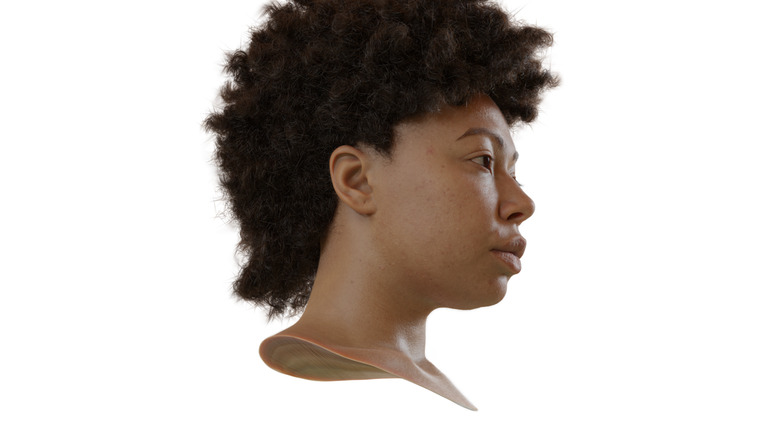
\includegraphics[width=\linewidth]{images/renders/khady_rgb_31.jpg}
  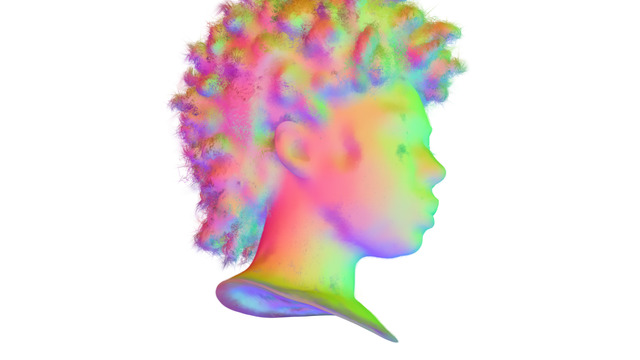
\includegraphics[width=\linewidth]{images/normals/khady_normals_31.jpg}
  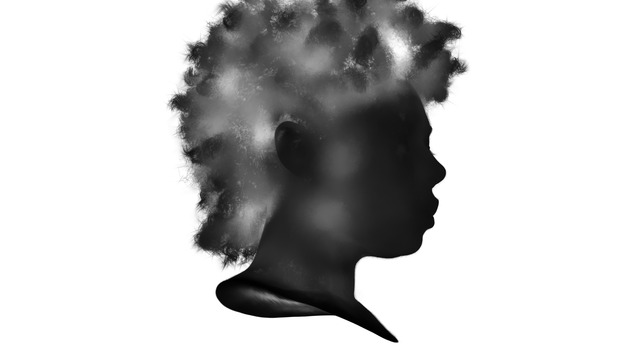
\includegraphics[width=\linewidth]{images/frosting_size/khady_size_31.jpg}
  \end{subfigure}
  %
  \hfill
  %
  \begin{subfigure}{0.155\linewidth}
  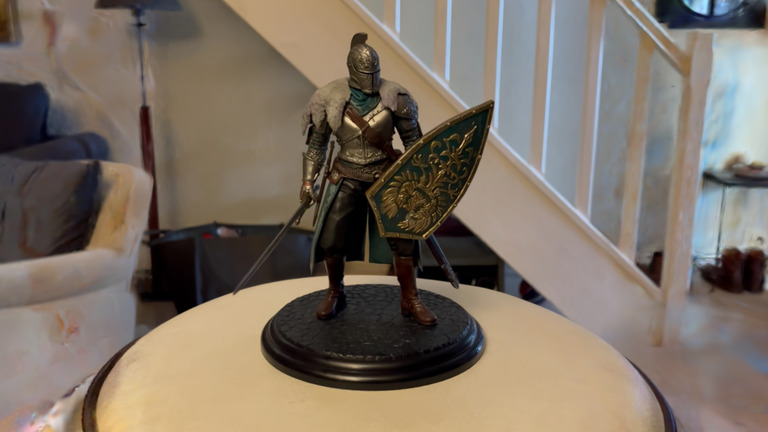
\includegraphics[width=\linewidth]{images/renders/faraam0_rgb_14.jpg}
  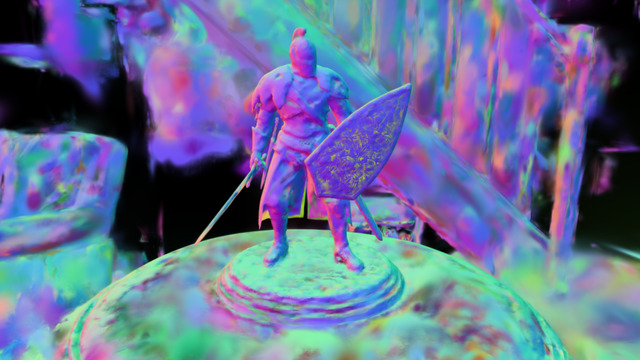
\includegraphics[width=\linewidth]{images/normals/faraam0_normals_14.jpg}
  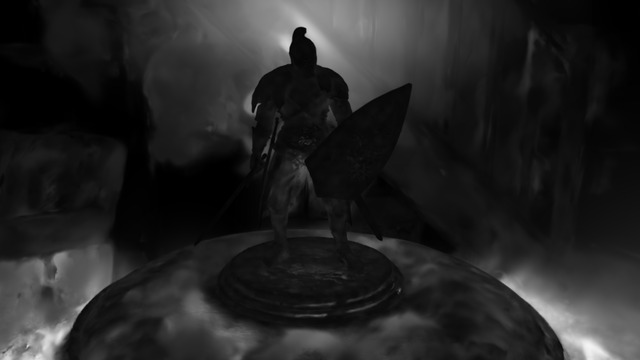
\includegraphics[width=\linewidth]{images/frosting_size/faraam0_size_14.jpg}
  \end{subfigure}
  %
  \hfill
  %
  \begin{subfigure}{0.155\linewidth}
  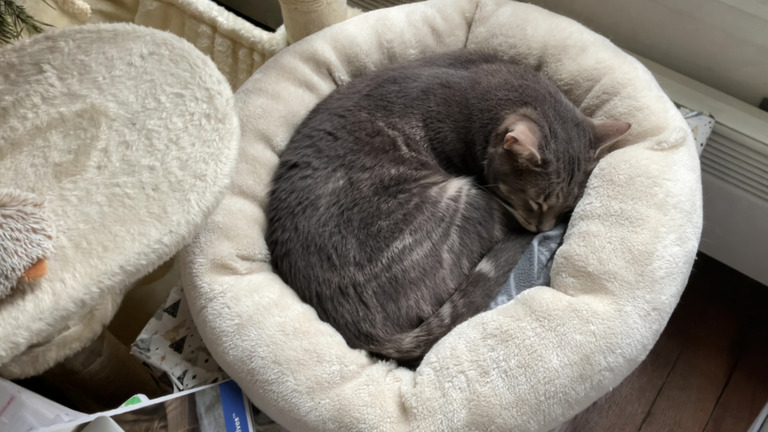
\includegraphics[width=\linewidth]{images/renders/sirius1_rgb_52bis.jpg}
  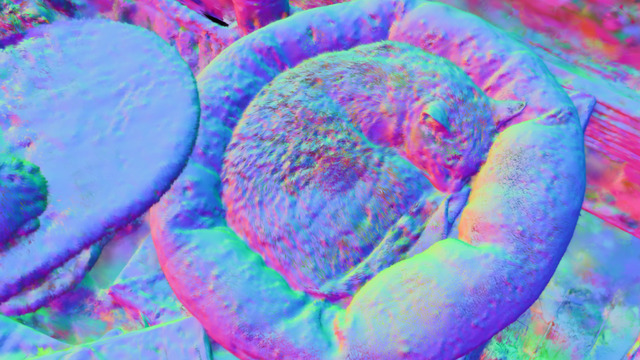
\includegraphics[width=\linewidth]{images/normals/sirius1_normals_52_bis.jpg}
  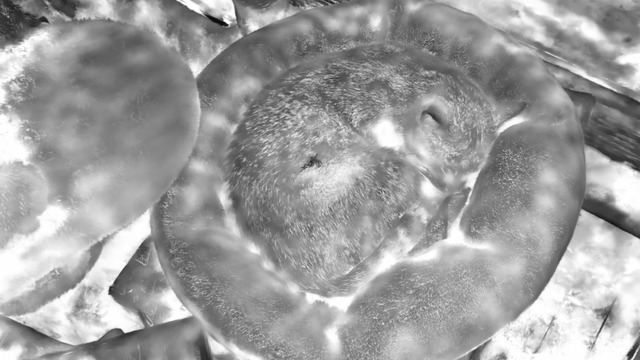
\includegraphics[width=\linewidth]{images/frosting_size/sirius1_size_52_ter.jpg}
  \end{subfigure}
  %
  \hfill
  %
  \begin{subfigure}{0.155\linewidth}
  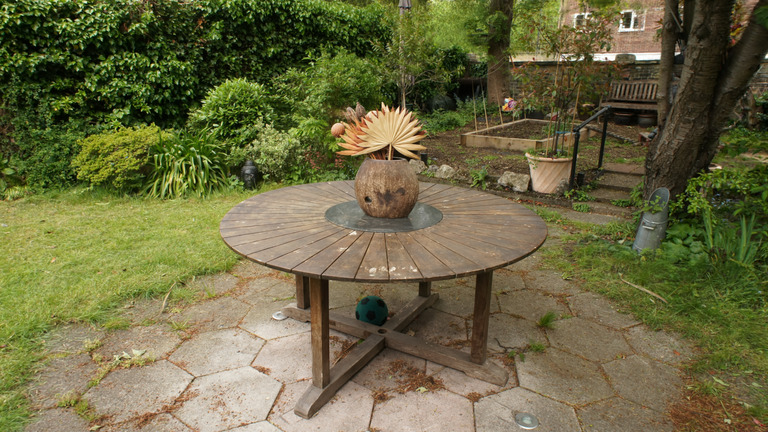
\includegraphics[width=\linewidth]{images/renders/garden_rgb_31.jpg}
  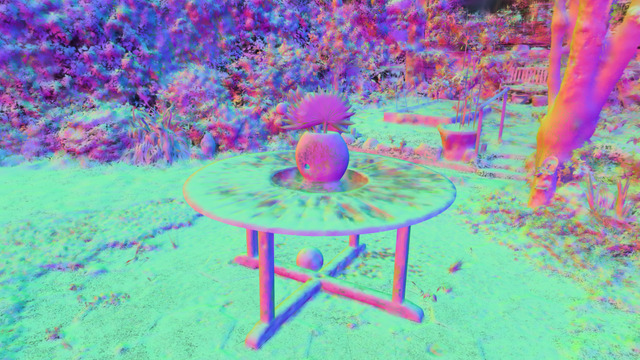
\includegraphics[width=\linewidth]{images/normals/garden_normals_31bis.jpg}
  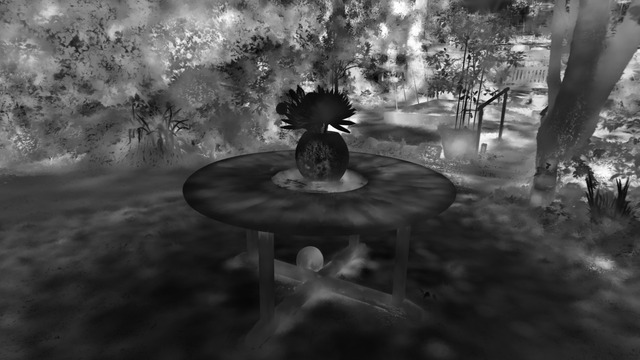
\includegraphics[width=\linewidth]{images/frosting_size/garden_size_31bis.jpg}
  \end{subfigure}
  %
  \hfill
  %
  \begin{subfigure}{0.155\linewidth}
  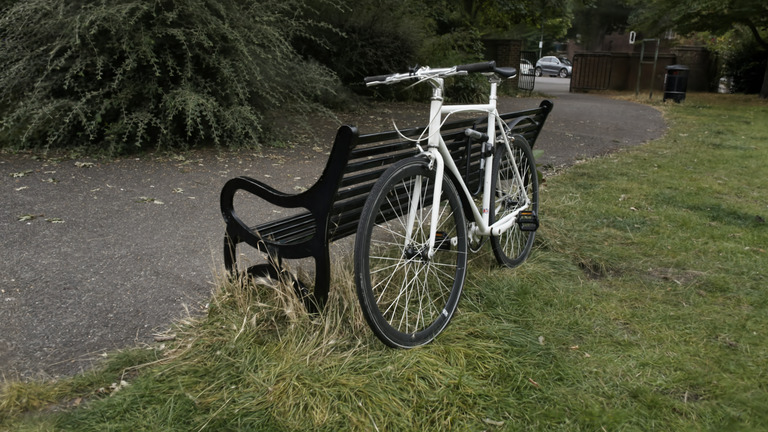
\includegraphics[width=\linewidth]{images/renders/bicycle_rgb_52.jpg}
  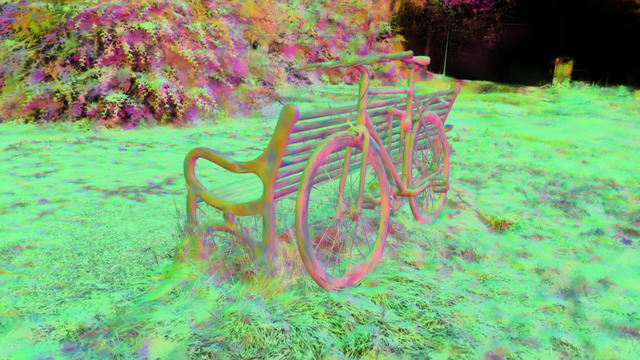
\includegraphics[width=\linewidth]{images/normals/bicycle_normals_52bis.jpg}
  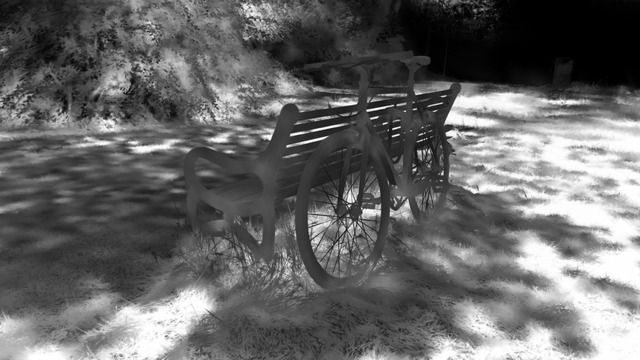
\includegraphics[width=\linewidth]{images/frosting_size/bicycle_size_52bis.jpg}
  \end{subfigure}
  %
  \caption{
  \textbf{Rendering complex scenes with Frosting.} First row: Renderings, Second row: recovered normal maps, Third row: estimated Frosting thickness. Note that the Frosting is thick on fuzzy materials such as the hair and the grass, as expected, and very thin on flat surfaces such as the table on the fourth column.
  }
  \label{fig:frosting-renders}
\end{figure}


\subsection{Frosting Optimization}

Once we constructed the outer and inner bounds of the Frosting layer, we initialize a densified set of Gaussians inside this layer and optimize them using 3DGS rendering loss as the unconstrained Gaussians. To make sure the Gaussians stay inside the frosting layer during optimization, we introduce a new parameterization of the Gaussians. Moreover, this parameterization will make possible to 
easily adjust the Gaussians' parameters when editing the scene.


\subsubsection{Parameterization.} Let us consider a triangular face of the base mesh $\calM$, with vertices denoted by~$\vec{v}_0, \vec{v}_1$, and~$\vec{v}_2$ and their corresponding normals~$\vec{n}_0, \vec{n}_1$, and~$\vec{n}_2$. After extracting inner and outer shifts from unconstrained Gaussians, we obtain six new vertices $(\vec{v}_i+\innershift_i \vec{n}_i)_{i=0,1,2}$ and $(\vec{v}_i+\outershift_i \vec{n}_i)_{i=0,1,2}$ that respectively belong to the inner and outer bounds of the frosting.
%
Specifically, these six vertices delimit an irregular triangular prism. We will refer to such polyhedrons as ``prismatic cells''. 
%
We parameterize the 3D mean~$\mu_g\in \IR^3$ of a Gaussian~$g \in \calG$ located inside a prismatic cell with a set of six barycentric coordinates split into two subsets~$(b_g^{(i)})_{i=0,1,2}$ and $(\beta_g^{(i)})_{i=0,1,2}$, such that 
%
\begin{equation}
    \mu_g = \sum_{i=0}^2 \left(
    b_g^{(i)} \left(\vec{v}_i+\outershift_i \vec{n}_i\right) +
    \beta_g^{(i)} \left(\vec{v}_i+\innershift_i \vec{n}_i\right)\right) \> ,
    \label{eq:barycentric-coordinates}
\end{equation}
%
with barycentric coordinates verifying $\sum_{i=0}^2 ( b_g^{(i)}+\beta_g^{(i)}) = 1$.
%
Using barycentric coordinates enforces Gaussians to stay inside their corresponding prismatic cell, and guarantees the stability of our representation during optimization.
%
In practice, we apply a softmax activation on the parameters to optimize to obtain barycentric coordinates that sum up to 1. 

\subsubsection{Initialization.} For a given budget $N$ of Gaussians provided by the user, we initialize $N$ Gaussians in the scene by sampling $N$ 3D centers $\mu_g$ in the frosting layer. Specifically, for sampling a single Gaussian, we first randomly select a prismatic cell with a probability proportional to its volume. Then, we sample random coordinates that sum up to 1. 
This sampling allows for allocating more Gaussians in areas with fuzzy and complex geometry, where more volumetric rendering is needed. However, flat parts  in the layer may also need a large number of Gaussians to recover texture details. Therefore, in practice, we instantiate $N/2$ Gaussians with uniform probabilities in the prismatic cells, and $N/2$ Gaussians with probabilities proportional to the volume of the cell.

We initialize the colors of the Gaussians with the color of the closest Gaussian in the unconstrained representation. However, we do not use the unconstrained Gaussians to initialize opacity, rotation, and scaling factors, as in practice, following the strategy from 3DGS~\cite{kerbl3Dgaussians} for these parameters provides better performance: 
We suppose the positions and configuration of the Gaussians inside the Frosting layer are already a good initialization, and resetting opacities, scaling factors and rotations helps Gaussians to take a fresh start, avoiding a potential local minimum encountered by previous unconstrained Gaussians.

Our representation allows for a much better control over the number of Gaussians than the original Gaussian Splatting densification process, as it is up to the user to decide on a number of Gaussians to instantiate in the frosting layer. These Gaussians will be spread in the entire frosting in a very efficient way, adapting to the need for volumetric rendering in the entire scene.

\subsubsection{Optimizing the Gaussian Frosting.} We reload the unconstrained Gaussians and apply our method for computing the inner and outer bounds of the Frosting. Then, for a given budget of $N$ Gaussians, we initialize $N$ Gaussians in the Frosting and optimize the representation while keeping the number of Gaussians constant. Note that compared to Vanilla 3DGS, this allows to control precisely the number of Gaussians.


\subsubsection{Editing, Deforming, and Animating the Frosting.} When deforming the base mesh, the positions of Gaussians automatically adjust in the frosting layer thanks to the use of the barycentric coordinates. 
%
To automatically adjust the rotation and scaling factors of the Gaussians, we propose a strategy different from the surface-based adjustment from SuGaR: In a given prismatic cell with center $\vec{c}$ and vertices $\vec{v}_i$ for $0\leq i<5$, we first estimate the local transformation at each vertex $\vec{v}_i$ by computing the rotation and rescaling of the vector $(c - \vec{v}_i)$. 
%
Then, we use the barycentric coordinates of a Gaussian $g$ to compute an average transformation at point $\mu_g$ from the transformation of all 6 vertices, and we adjust the rotation and scaling factors of $g$ by applying this average transformation. 
%
Please note that the spherical harmonics are also adjusted in practice, to ensure the consistency of the emitted radiance depending on the averaged rotation applied to the Gaussian.
%
We provide more details about this automatic adjustment of Gaussian parameters in the supplementary material.
\section{Experiments}

\subsection{Experimental setup}

Our experiments all use the Llama \citep{Llama} architecture trained on WikiText-103~\citep{WikiText103} (excepting the large-scale runs in \Cref{sec:fp8_training}). We apply current best-practice LLM training techniques from the literature (full settings are given in \Cref{tab:experiment_defaults}). In accordance with our analysis of settings for \mut\ in \Cref{sec:challenges:mut}, we remove parameters from norm layers, use independent AdamW, and avoid training on too many epochs for both \umup\ and \mup\ for the sake of fair comparison.

\subsection{Quantifying hyperparameter interdependence} \label{sec:experiments:hp_independence}

Our principled approach to HPs (\Cref{sec:umup:principled_hps}) contains the requirement that their optimal values should depend minimally on the value of other HPs. We now investigate this empirically, conducting a 2D sweep over every pair of HPs for \mup\ and \umup, shown in \Cref{fig:additional_experiments:mult_grid_mup,,fig:additional_experiments:mult_grid_umup} respectively.

To derive an empirical measure of HP dependency, we introduce the notion of \textit{transfer error} (see \Cref{alg:transfer_error}). This considers a pair of HPs, with one `fixed' and the other for `transfer'. We take the best value of the transfer HP for each non-optimal value of the fixed HP, and use it with the optimal value of the fixed HP. The transfer error is the difference between the losses obtained and the minimum loss. \Cref{fig:experiments:transfer_error} shows this measure for each pair of HPs under \mup\ and \umup, reflecting the improvement in HP dependency as a result of our scheme. This gives \umup\ a reduced risk of small transfer errors leading to large degradations, and the potential to sweep HPs in a more separable way.

\begin{figure}[t]
    \vspace{-1em}
    \centering
    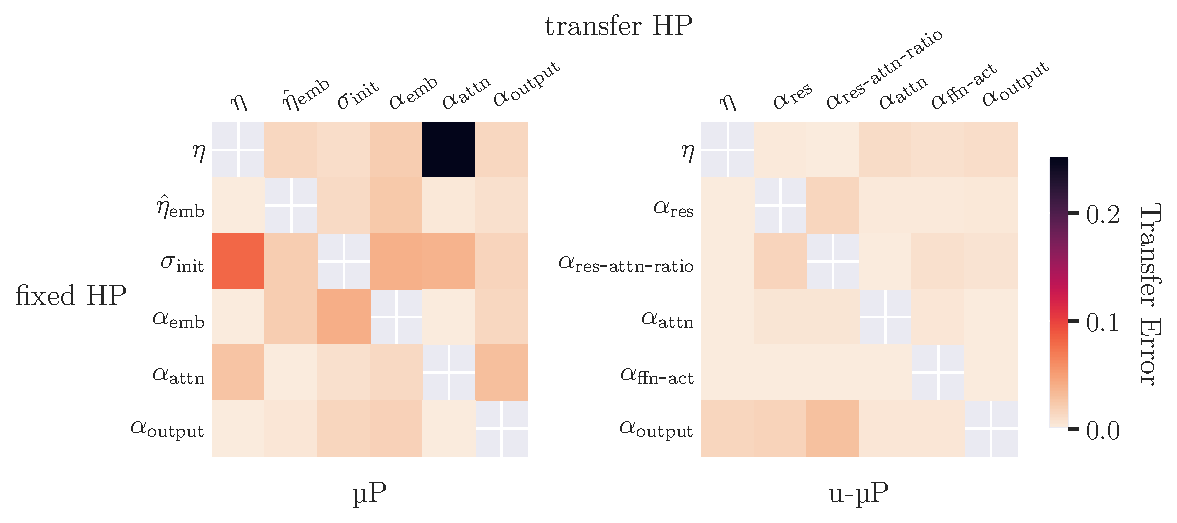
\includegraphics[width=\textwidth]{arXiv/figures/hp_pair_dependencies_val.pdf}
    \caption{A visualization of the dependencies between pairs of HPs under each scheme. Transfer error measures the extent to which the optimal value of the transfer HP depends on the fixed HP (see \Cref{alg:transfer_error}). On average, \mup\ has a transfer error of 0.03, whereas \umup\ has 0.005.}
    \label{fig:experiments:transfer_error}
\end{figure}

\subsection{Hyperparameter search} We now leverage this improved separability of HPs for the purpose of efficient sweeping. In \Cref{fig:fig1}~(a) we conduct a standard random search for \mup\ and \umup, along with the independent search outlined in \Cref{sec:umup_hp_search} (and \Cref{app:umup_hp_search_algorithm}). We observe the following:

\begin{enumerate}
    \item For \umup\ the LR-sweep phase of independent search alone is sufficient to reach near-optimal loss (totaling 9 runs). During this phase other HPs are fixed at 1, which for \umup\ means that the inputs to operations are generally unit-scaled.

    \item Consequently, we conclude that unit scale at initialization is close to the ideal scaling for effective learning here. This is not a property we asserted a priori, nor do we argue that it necessarily holds for other training setups and models; hence why we still provide a set of extended HPs to be swept.

    \item In contrast \mup\ still requires non-LR HPs to be swept to attain a reasonable loss. Unlike \umup, fixing HPs at 1 results in arbitrarily-scaled inputs, which appear to result in worse training.

    \item The `combined mults' phase causes the loss to spike for \mup. This is due to the HP dependencies shown in \Cref{fig:experiments:transfer_error}, which mean HPs cannot be swept independently and used together. Conversely, lower dependence means this can be done for \umup, making random search unnecessary.
\end{enumerate}

\subsection{Hyperparameter transfer}

% As \umup\ follows the \mup\ parametrization rules (with the exception of the embedding LR scaling rule in \Cref{sec:umup:emb_lr_rule}), we still expect it to satisfy the transfer properties of \mup. In fact, \umup's transfer properties are generally better than those of the \mup\ baseline, thanks to our unit-scale criterion and careful HP design.

We demonstrate the transfer of LR across width in \Cref{fig:fig1} (b), of the other extended HPs across width in \Cref{fig:lr_transfer}, and of LR across training steps, batch size and depth in \Cref{fig:experiments:hp_transfer_over_width}. We find that:

\begin{enumerate}
    \item The optimal LR is constant for all widths under \umup, from 128 to 4096.

    \item The optimal LR is also approximately constant for training steps, batch size and depth. This means we can scale our proxy model down across all these axes and maintain LR transfer. Of these, width appears the most stable and depth the least.

    \item Whereas \mup\ sees diminishing returns for larger widths, \umup\ continues to benefit from width, with the 2048 \umup\ model matching the 4096 \mup\ model. We attribute this primarily to our improved embedding LR rule.

    \item Non-LR HPs also have approximately constant optima across width under \umup. This is not true for \mup, where $\hat{\eta}_\mathrm{emb}$ has poor transfer due to the embedding scaling rule issue identified in \Cref{sec:umup:emb_lr_rule}, along with $\sigma_\mathrm{init}$ which in \Cref{sec:challenges:which_hps} we argue should not be grouped across all weights (and drop from the \umup\ HP scheme).

    \item The optimal values found for non-LR HPs are all close to 1. In practice this means that dropping these HPs entirely is potentially viable for similar models and training setups.
\end{enumerate}

\begin{figure}[t]
    \centering
    \begin{subfigure}{\textwidth}
        \centering
        \includegraphics[width=\textwidth]{arXiv/figures/lr_transfer_mup.pdf}
    \end{subfigure}
    \begin{subfigure}{\textwidth}
        \centering
        \includegraphics[width=\textwidth]{arXiv/figures/lr_transfer_u-mup.pdf}
    \end{subfigure}
    \caption{Learning rate transfer for \mup{} (top) and \umup{} (bottom), over training steps, batch size and depth. See \Cref{fig:fig1}~(b) for transfer over width. The \textbf{default} shape parameter for other panels is shown in bold. The shaded area shows the $95\%$ confidence interval for the mean.}
    \label{fig:lr_transfer}
\end{figure}

\subsection{FP8 training} \label{sec:fp8_training}

In this section we justify the simple mixed-precision scheme described in \Cref{sec:umup:low_prec_training} and demonstrate that it can be used to train \umup\ models out-of-the-box.

\paragraph{Proof-of-concept} \Cref{fig:numerics:scale} shows the RMS of all linear layer inputs for a moderately sized transformer. RMS captures the larger of the mean and scale of a distribution, and as such is a good test of whether a tensor is likely to suffer over/underflow in low-precision. We observe that \umup\ tensors largely have RMS starting close to $1$ and remaining so at the end of training, supporting our scheme.

\Cref{fig:numerics:rms_during_training} demonstrates the scale-growth of critical tensors which our scheme is designed to accommodate, showing RMS on a per-tensor basis over steps. \Cref{fig:numerics:scale_scaling} provides further insight into this issue, showing the effect of LR, width, depth, steps and batch size on the RMS of critical tensors.

As an initial proof-of-concept we train a \umup\ model using our FP8 scheme over 8k steps, using HPs from a proxy model, as shown in \Cref{fig:fig1}~(c). We see only a small degradation versus FP32, and at this scale critical tensors can still be cast to FP8 using \texttt{E5M2}, while gradients can even use \texttt{E4M3}.

%\subsection{Numerical properties} \label{subsec:numerical_properties}

%,  Detailed analysis of these statistics is given in \Cref{app:fp8_training}, with our results supporting the central thesis of Unit Scaling: that tensors are well-scaled at initialization and largely remain so across training.

%Based on these conclusions we propose our primary FP8 scheme: for every matrix multiplication, we cast the input, weight and grad-output tensors to \texttt{E4M3}, with the exception of the inputs to FFN and self-attention final projections, which are cast to \texttt{E5M2} to accommodate their growing scale. This simply requires FP8 casts to be inserted into the model, avoiding the more complex scaling techniques used for FP8 in the literature (see \Cref{app:low_precision_and_its_trade_offs}). This is possible due to the numerical stability we see in our analysis of \umup. Additional details of our primary FP8 scheme are given in \Cref{app:fp8_scheme}.

%As we demonstrate in \Cref{subsec:large_scale}, the primary scheme needs to be slightly adapted when model size, sequence length and number of training steps increase substantially. 

%\subsection{FP8 training at smaller scale} \label{sec:experiments:fp8}

%We now show that \umup\ can indeed be trained in our primary FP8 scheme in a smaller-scale setting (in terms of training tokens, rather than model-size). We note that our aim here is a proof-of-concept that this form of low-precision training can be done without degradation, not a demonstration of improved throughput which we leave to future work. To investigate the question of the potential benefits of FP8 training, \Cref{app:scaled_mm_benchmarking} shows results for micro-benchmarking low-precision matmuls. We find that the addition of scaling factors adds no overhead, making our \umup\ modifications essentially `free'.

%\Cref{fig:fig1} (c) demonstrates the application of our FP8 scheme to model-training at width 4096. We use exactly the HPs suggested by the sweep in \Cref{fig:fig1} (a), but transferred to the larger model-width. \mup\ fails entirely under our FP8 scheme due to gradient underflow, reflecting the requirement for different, and likely more complex scaling scheme. In contrast, \umup\ trains in FP8 with only a small increase in validation loss versus the full-precision baseline.

\begin{figure}[t]
    \centering
    \begin{subfigure}{.46\textwidth}
        \centering
        \includegraphics[width=\textwidth]{arXiv/figures/rms_at_init.pdf}
    \end{subfigure}
    \begin{subfigure}{.46\textwidth}
        \centering
        \includegraphics[width=\textwidth]{arXiv/figures/rms_end_training.pdf}
    \end{subfigure}
    \caption{Per-tensor $\mathrm{RMS} = \sqrt{\sigma^2 + \mu^2}$ across \umup\ and \mup\ models at initialization (left) and after training (right). \umup\ tensors have RMS that starts close to $1$ and remains within E4M3 range at the end of training. Dashed and solid red lines show each format's min. normal and subnormal values.}
    \label{fig:numerics:scale}
\end{figure}

%\subsection{FP8 training at large-scale} \label{subsec:large_scale}

\paragraph{Larger scale} Next we consider a more realistic training scenario \footnote{The training codebase used for our larger-scale experiments can be found at the following url \url{https://github.com/Aleph-Alpha/scaling}. We have also released model checkpoints, which are available at \url{https://huggingface.co/Aleph-Alpha}.}.
% \footnote{The large scale experiments were run on a separate code base optimized for distributed training that will be made available in the near future.}
Using the same architecture, and following the steps set out in our \umup\ user-guide (\Cref{app:using_umup_guide}), we train our target models on 300B tokens of the SlimPajama dataset \citep{SlimPajama} (see \Cref{app:large_model_training} for training details).

We begin with an independent search (\Cref{sec:umup_hp_search}) over our \umup\ proxy model's HPs. Here we make the following observations:
\begin{enumerate}
    \item When using a relatively small proxy model (8 layers and 512 width), the HP-loss landscape is rather noisy. By doubling the width we can discern optimal HP values more clearly.
    \item The most important HPs are $\eta$ and $\alpha_\mathrm{res\text{-}attn\text{-}ratio}$. All others can be left at the default of $1$.
    \item The optimal values of these HPs are $\eta = 2^{3.5}$ and $\alpha_\mathrm{res\text{-}attn\text{-}ratio} = 2^{-2.0}$ and thus differ non-trivially from the observed HPs in our smaller-scale experiments.
\end{enumerate}

We then train \umup\ models of approximately 1B, 3B and 7B parameters, using our FP8 mixed-precision scheme (see \Cref{sec:umup:low_prec_training}). We also train two baselines at each size: the first is a BF16 version of our \umup\ models, and the second is a set of SP models using the weight init scheme from the Pythia model family~\citep{Pythia} and the LR scheme from Llama 3~\citep{LLAMA3}, scaling inversely with width and using a LR of 3e-4 at 7B scale.
The loss curves are shown in \Cref{fig:scaleup}. All FP8 runs converge and show no significant loss degradation. In comparison to SP, the \umup\ models have a qualitatively different training curve with a higher loss for most of training that catches up in latter stages, hinting at a fundamentally different optimization trajectory. In terms of downstream performance, both of the \umup\ 7B models are competitive with SP. In particular, the scores of the FP8 model are mostly on par with the BF16 models (see \Cref{tab:eval_results}).

%We also record the magnitude of tensors in the model during training (\ce{TODO: include figure }). Some of the critical layers show a significant scale growth over time, which makes it impossible to naively cast them to FP8. On the other hand, the non-critical tensor scales are very stable across training time, and model size. This is strong evidence for \umup\ FP8 to work at even larger scales.

% . We also observe that using purely the \texttt{E4M3} format in the `non-problematic' layers leads to divergence as well, whereas the hybrid scheme of using \texttt{E4M3} for the activation and the weight and \texttt{E5M2} for the output gradient is stable.
%To tackle the layers that exhibit scale growth, we fit them with a lightweight form of dynamic rescaling, leaving the rest of the model untouched. 

%The dynamic rescaling works as follows: Before the matrix multiplication, we normalize the input by its standard deviation and divide the result by the same scale afterwards, while ignoring both of these operations in the backward computation. We emphasize that this is still considerably less complex than the per-tensor scaling strategy that is usually required for FP8 training.

%Using this refined FP8 scheme we perform two series of experiments:
%\begin{enumerate}
  %  \item On the 1B scale, we train a comparable SP model adopting the learning rate and initialization scheme from the Pythia model family~\citep{Pythia}, which we consider a strong established baseline. Apart from a standard training in BF16 mixed precision, we also try a simple FP8 cast and the Nvidia Transformer Engine framework~\citep{Transformer_Engine} for this baseline. We then compare these SP models to three variants of our \umup\ 1B model: One model in mixed precision, one model casting all layers except the critical ones to FP8 (our `partial' scheme in \Cref{fig:scaleup}), and one where we apply our full FP8 scheme. Overall the \umup\ models perform favorably  (see \Cref{fig:scaleup} (left)).
   % \item We train FP8 models up to 7B parameters using our full FP8 scheme. All runs converge (see \Cref{fig:scaleup} right), and we expect our method to work at larger scales still.
%\end{enumerate}


%We then train our target models using this FP8 scheme in \Cref{fig:dynamic_rescaling_losses}. At each model-size we demonstrate successful FP8 training, and expect it to work at larger scales still.

%\begin{figure}[t]
  %  \centering
  %  \begin{subfigure}{\textwidth}
  %      \centering
  %      \includegraphics[width=\textwidth]{arXiv/figures/fig_scaleup.pdf}
  %  \end{subfigure}
  %  \caption{(Left) Comparison of 1B training curves for \umup\ and SP, using BF16 mixed precision vs FP8. Directly casting to FP8 causes SP to diverge, whereas \umup\ still converges and outperforms the Transformer Engine FP8 baseline (SP FP8 T.E.). Using our proposed partial FP8 scheme, \umup\ maintains nearly full performance compared to BF16 mixed precision. (Right) Loss curves from large scale training runs up to 7B using the \umup\ FP8 scheme. Both figures use a smoothed running average loss with window size 100.}
  %  \label{fig:scaleup}
%\end{figure}

\begin{figure}[t]
    \vspace{-1.5em}
    \centering
    \begin{subfigure}{0.4\textwidth}
        \centering
        \includegraphics[width=\textwidth]{arXiv/figures/large_scale_BF16_vs_FP8.pdf}
    \end{subfigure}
    \hspace{2em}
    \begin{subfigure}{0.4\textwidth}
        \centering
        \includegraphics[width=\textwidth]{arXiv/figures/large_scale_umup_vs_sp.pdf}
    \end{subfigure}
    \vspace{-0.5em}
    \caption{Large-scale training runs. (Left) \umup\ BF16 vs \umup\ FP8. (Right) \umup\ BF16 vs SP BF16.}
    \label{fig:scaleup}
\end{figure}

\begin{table}[t] 
  \centering
  \caption{0-shot benchmark results at 7B scale.}
\begin{tabular}{llcccccc}
\toprule
Scheme & Format & MMLU & HellaSwag & OpenBook QA & PIQA & TriviaQA & WinoGr \\
\midrule
SP & BF16 & 29.6 & 52.4 & 27.8 & 76.5 & 22.2 & 63.3 \\
\umup\ & BF16 & 29.0 & \textbf{53.4} & \textbf{31.6} & 77.1 & \textbf{23.4} & 63.7 \\
\umup\ & FP8 & \textbf{31.2} & \textbf{53.4} & 29.6 & \textbf{77.6} & 21.3 & \textbf{65.7} \\
\bottomrule
\label{tab:eval_results}
\vspace{-1.5em}
\end{tabular}
\end{table}




  %To a Results for this can be seen in \todocite. We observe a small benefit in using non-unit values for the $\mathord{?}$ and $\mathord{?}$ HPs, as well as a slightly different optimal LR ($\mathord{?}$ instead of $2^{1.5}$).

%Transferring these HPs to our target models, we train SP and \umup\ models at the 1B, 3B and 7B scale, with and without FP8, as shown in figure \todocite. Using our transferred HPs, our \umup\ models match the SP baselines, and unlike the SP models can be trained using a simple FP8 scheme. This differs slightly from our primary FP8 scheme as the two activation tensors that exhibit scale-growth require dynamic scaling (see \Cref{app:large_model_training}), though the large majority of tensors still use our un-scaled FP8 cast. This demonstrates that our scheme can be applied effectively to LLMs in realistic training settings.

%[add any additional details here, and to corresponding Appendix A section once figures are ready]

\section{Discussion}
% \subsection{Concurrent Work}
% In recent years it has become more popular to release ``uncensored'' language models, and with that there have been tools and techniques developed to detect undesirable outputs produced by these models. One such tool is Llama Guard \cite{inan2023llama}, a large language model designed to perform both prompt- and response-classification to maximise the safety of chat systems. Like DPH, Llama Guard can be used to detect and reject harmful outputs produced by a language model. However, unlike DPH, Llama Guard is an entirely separate model which must be run concurrently with chat model and therefor increases the compute and memory requirements of the combined system. % this especially contrasts with DPH being especially suited for small language models which inherently require a much smaller compute budget.

\subsection{Future Work}
As shown in the results section, DPH is capable of learning to assign higher rewards to preferred outputs and lower rewards to dispreferred outputs which implies the pooling function learns rich features with respect to prompt-completion pairs. We believe that it would be possible to also extract additional information from the output of the pooling function to detect finer grained signals such as helpfulness, humor, creativity, toxic content, etc. This can be achieved by training on a conversational dataset such Open Assistant \cite{köpf2023openassistant} which contains a variety of human-curated labels in addition to machine-generated labels produced by Detoxify \cite{Detoxify}.

% It is also worth examining how the performance of DPH scales with larger language models, and if it can be used as a post-hoc technique to provide safety guardrails for uncensored language models such as Mistral 7B and observe how it performs compared to systems such as Llama Guard while maintaining much lower compute requirements.

\subsection{Limitations}
The main benefit of DPH being its ability to perform alignment without directly effecting the model's output distribution is also its main limitation: unlike other alignment techniques which can help prevent the model generating harmful outputs, DPH is only capable of \textit{detecting} harmful outputs. Although we do include DPO alignment in our experiments to reduce the likelihood of harmful outputs, DPH does not require such model alignment to function, which shifts the responsibility of rejecting harmful outputs to the end user or service provider.

\subsection{Conclusion}
In this paper we introduced Direct Preference Heads, a novel form of language model alignment which is performed at inference time to prune candidate completions for a given prompt. Unlike other alignment techniques which coerce the model into generating human preference aligned outputs, DPH instead produces reward scores for candidate outputs without affecting the actual generation process and therefor avoids the issue of RLHF leading to degraded performance when applied to smaller language models. We formulated two loss functions for DPH and find strong connections to Conservative DPO, implying that DPH is robust to label noise and can be tuned to a specific confidence margin. Finally, we evaluated our methods on a number of NLU, commonsense reasoning and reading Comprehension tasks and found that DPH is able to consistently outperform both our SFT baseline and multiple publicly available language model checkpoints of varying size and training volume.

\subsection*{Broader Impacts}
As with all language modeling systems we cannot guarantee all responses produced by our models are factually correct nor can we guarantee that they are safe and free from harmful content. Our work focuses on creating a system that helps filter out incorrect and harmful messages by scoring candidate outputs, but as with all alignment techniques our models may be susceptible to so-called `jailbreaks' which can coerce the model into incorrectly assigning a higher score to less desirable content. To maximise safety DPH should be implemented alongside other safety guardrails such as Llama Guard \cite{inan2023llama} when used for publicly facing chat systems, and we intend for our provided model checkpoints to be used for reproduction of results and further research in the field of alignment.
\newpage

% ---- Bibliography ----
%
% BibTeX users should specify bibliography style 'splncs04'.
% References will then be sorted and formatted in the correct style.
%
\bibliographystyle{splncs04}
\bibliography{arxiv}

\newpage
\centerline{\large Supplementary Material}

\vspace{0.3in}
\noindent
In this supplementary material, we provide the following elements:
\begin{itemize}
    \item A description of our method to improve the surface reconstruction from SuGaR~\cite{guedon2023sugar}.
    \item Additional details about our strategy to initialize the Frosting layer and automatically adjust Gaussians' parameters when deforming, editing, or animating our representation.
\end{itemize}
% TODO
We also provide a \href{https://anttwo.github.io/frosting/}{\underline{video}} that offers an overview of the approach and showcases additional qualitative results. Specifically, the video demonstrates how Frosting can be used to edit, combine or animate Gaussian Splatting representations.

\setcounter{section}{+6}
\section{Improving surface reconstruction}

% \subsubsection{Improving surface reconstruction.} 

We improve the surface reconstruction method from SuGaR by proposing a way to automatically adjust the hyperparameter of the Poisson surface reconstruction~\cite{kazhdan-2006-poissonsurfacereconstruction} stage.

Poisson surface reconstruction first recovers an underlying occupancy field $\chi:\IR^3\mapsto [0,1]$
and applies a marching algorithm on $\chi$, which allows for a much better mesh reconstruction than the density function. This approach allows for high scalability as the marching algorithm is applied only in voxels located close to the point cloud. 

To estimate $\chi$, Poisson surface reconstruction discretizes the scene into $2^D \times 2^D \times 2^D$ cells by adapting an octree with depth $D\in \IN$ to the input samples.  $D$ is a hyperparameter provided by the user: The higher $D$, the higher the resolution of the mesh.

By default, SuGaR~\cite{guedon2023sugar} uses a large depth $D=10$ for any scene, as it guarantees a high level of details. However, if the resolution is too high with respect to the complexity of the geometry and the size of the details in the scene, the shapes of the Gaussians become visible as ellipsoidal bumps on the surface of the mesh, and create incorrect bumps or self-intersections. More importantly, holes can also appear in the geometry when $D$ is too large with regards to the density of the Gaussians and the sampled point cloud.

% However, depending on the spatial extent of the scene, on the complexity of the geometry, or even on the distance between the camera and the objects to reconstruct, a parameter $D$ that is too large can produce artifacts in the scene, as shown in Figure~\ref{fig:mesh-comparison} and mentioned in GitHub issues of SuGaR's implementation. 


We therefore introduce a method to automatically select $D$. A simple strategy would be to adjust the depth of the octree such that the size of a cell is approximately equal or larger than the average size of the Gaussians in the scene, normalized by the spatial extent of the point cloud used for reconstruction. Unfortunately, this does not work well in practice: We found that whatever the scene (real or synthetic) or the number of Gaussians to represent it, Gaussian Splatting optimization systematically converges toward a varied collection of Gaussian sizes, so that there is no noticeable difference or pattern in the distribution of sizes between scenes.

We noticed that the distance between Gaussians is much more representative of the geometrical complexity of the scene and thus a reliable cue to fix $D$. Indeed, a large but very detailed shape can be reconstructed using Gaussians with large size, if these Gaussians are close to each other. On the contrary, whatever their size, if the centers of the Gaussian are too far from each other, then the rendered geometry will look rough. 

Consequently, to first evaluate the geometrical complexity of a scene, we propose to compute, for each Gaussian $g$ in the scene, the distance between $g$ and its nearest neighbor Gaussian. We use these distances to define the following geometrical complexity score $CS$:
%
\begin{equation}
    CS = Q_{0.1} \left( \left\{\min_{g'\neq g} \frac{\|\mu_g - \mu_{g'}\|_2}{L}\right\}_{g\in \calG} \right) \> ,
    \label{eq:complexity_score}
\end{equation}
%
where $\calG$ is the set of all 3D Gaussians in the scene, $L$ is the length of the longest edge of the bounding box of the point cloud to use in Poisson reconstruction, and $Q_{0.1}$ is the function that returns the 0.1-quantile of a list. We use the 0.1-quantile rather than the average because Gaussians that have a neighbor close to them generally encode details in the scene, which provide a much more reliable and less noisy criterion than using the overall average. We also use a quantile rather than a minimum to be robust to extreme values. In short, this complexity score $CS$ is a canonical distance between the closest Gaussians in the scene, i.e., the distance between neighbor Gaussians that reconstruct details in the scene. 

% \input{figures/complexity_score}

Since the normalized length of a cell in the octree is $2^{-\bar{D}}$ and this score represents a canonical normalized distance between Gaussians representing details in the scene, we can compute a natural optimal depth $\bar{D}$ for the Poisson reconstruction algorithm:
%
\begin{equation}
    \bar{D} = \lfloor -\log_2 \left(\gamma \times CS\right) \rfloor \> ,
    \label{eq:optimal-depth}
\end{equation}
%
where $\gamma > 0$ is a hyperparameter that does not depend on the scene and its geometrical complexity. This formula guarantees that the size of the cells is as close as possible but greater than $\gamma \times CS$. Decreasing the value of $\gamma$ increases the resolution of the reconstruction. But for a given $\gamma$, whatever the dataset or the complexity of the scene, this formula enforces the scene to be reconstructed with a similar level of smoothness. 

Choosing $\gamma$ is therefore much easier than having to tune $D$ as it is not dependent on the scene. 
In practice, we use $\gamma=100$ for all the scenes. Our experiments validates that this method to fix $D$ results in greater rendering performance.



\section{Initializing the frosting layer}

\subsection{Sampling Gaussians in the frosting layer} 

\subsubsection{Sampling more Gaussians in thicker parts of the frosting.} For a given budget $N$ of Gaussians provided by the user, we initialize $N$ Gaussians in the scene by sampling $N$ 3D centers $\mu_g$ in the frosting layer. Specifically, for sampling a single Gaussian, we first randomly select a prismatic cell with a probability proportional to its volume. Then, we sample random coordinates that sum up to 1. 
%
This sampling allows for allocating more Gaussians in areas with fuzzy and complex geometry, where more volumetric rendering is needed. However, flat parts  in the layer may also need a large number of Gaussians to recover texture details. Therefore, in practice, we instantiate $N/2$ Gaussians with uniform probabilities in the prismatic cells, and $N/2$ Gaussians with probabilities proportional to the volume of the cell.

\subsubsection{Contracting volumes in unbounded scenes.} In real unbounded scenes, 3D Gaussians located far away from the center of the scene can have a significantly large volume despite their limited participation in the final rendering. This can lead to an unnecessarily large number of Gaussians being sampled in the frosting layer far away from the training camera poses. To address this issue, we propose distributing distant Gaussians proportionally to disparity (inverse distance) rather than distance.

When sampling Gaussians in practice, we start by contracting the volumes of the prismatic cells. We achieve this by applying a continuous transformation $f:\IR^3 \rightarrow \IR^3$ to the vertices of the outer and inner bounds of the frosting layer. 
%
Then, we compute the volumes of the resulting ``contracted'' prismatic cells and use these adjusted volumes for sampling Gaussians within the frosting layer, as previously described. The transformation function $f$ aims to contract the volume of prismatic cells located far away from the center of the scene. We define $f$ using a formula similar to the contraction transformation introduced in Mip-NeRF~360~\cite{barron2022mipnerf360}:
\begin{equation}
    f(x) = \begin{cases}
        x & \text{if} \>\>\>\> \|x-c\| \leq l\\
        c + l \times \left(2 - \frac{l}{\|x-c\|}\right) \left(\frac{x-c}{\|x-c\|}\right) & \text{if} \>\>\>\> \|x-c\| > l
    \end{cases} \>,
    \label{eq:contraction}
\end{equation}
where $c\in \IR^3$ is the center of the bounding box containing all training camera positions, and $l\in\IR_+$ is equal to half the length of the diagional of the same bounding box. 
%
We choose the bounding box of the camera positions as our reference scale because both 3D Gaussian Splatting~\cite{kerbl3Dgaussians} and SuGaR~\cite{guedon2023sugar} use this same reference for scaling learning rates and distinguishing foreground from background in unbounded scenes.

\subsection{Avoiding self-intersections in the frosting layer}

In the main paper, we define the inner and outer bounds of the frosting layer by adding inner and outer shifts $\innershift_i$ and $\outershift_i$ to the vertices $\vec{v}_i$ of the base mesh. This results in two bounding surfaces with vertices $\vec{v}_i + \innershift_i$ and $\vec{v}_i + \outershift_i$. 
%
In practice, we wish to minimize self-intersections within the frosting layer, specifically avoiding prismatic cells intersecting with each other.

While self-intersections do not directly impact rendering quality, they can lead to artifacts during scene editing or animation. Consider the scenario where different cells intersect. In such cases, moving a specific triangle of the base mesh may not affect all Gaussians intersecting the surrounding cell: Some Gaussians may belong to prismatic cells associated with different triangles, resulting in artifacts due to their failure to follow local motion or scene edits.

To mitigate self-intersections, we adopt an indirect approach for initializing the shifts $\innershift$ and $\outershift$. 
Instead of using the final computed values directly, we start with shifts equal to zero and progressively increase them until reaching their final values. 
As soon as an inner vertex (or outer vertex) of a prismatic cell is detected to intersect another cell, we stop further increases in its inner shift (or outer shift). 
This straightforward process significantly reduces self-intersections in the frosting layer while maintaining rendering performance.

By following this approach, we ensure that the frosting layer remains free from unwanted artifacts while preserving efficient rendering capabilities.

\section{Adjusting Gaussians' parameters for edition}

When editing or animating the scene, we automatically adjust Gaussians' parameters. Specifically, in a given prismatic cell with center $\vec{c}$ and six vertices $\vec{v}_i$ for $0\leq i<6$, we first estimate the local transformation at each vertex $\vec{v}_i$ by computing the rotation and rescaling of the vector $(c - \vec{v}_i)$. 

To compute the local rotations at vertex $\vec{v}_i$, we use an axis-angle representation where the axis angle is the normalized cross-product between the previous and the current values of the vector $(c - \vec{v}_i)$.
%
The local rescaling transformation at vertex $\vec{v}_i$ is computed as the transformation that scales along axis $(c - \vec{v}_i)$ with the appropriate factor but leaves other axes unchanged.

To update the scaling factors and rotation of a Gaussian $g$, we first apply each of these six transformations on the three main axes of the Gaussian. We then average the resulting axes using the barycentric coordinates of the center $\mu_g$ of the Gaussian. We finally orthonormalize the three resulting axes.


\end{document}
